\documentclass[a4paper,12pt]{article}



% Pacotes essenciais
\usepackage[brazil]{babel}
\usepackage[T1]{fontenc}

% Pacotes para citações no estilo ABNT
\usepackage[alf]{abntex2cite}

% Pacotes adicionais
\usepackage{csquotes, graphicx, xcolor, comment, enumerate, multirow, 
    multicol, titlesec, amsmath, amsthm, amsfonts, amssymb, dsfont, 
    blindtext, ragged2e, array, enumitem, tikz, bbding, pifont, wasysym, 
    titling, longtable, fancyhdr, url, float, placeins, xurl}

\usepackage{graphicx}\usepackage[table]{xcolor}
% Configuração de margens
\usepackage[lmargin=2cm, rmargin=2cm, tmargin=2cm, bmargin=2.5cm]{geometry}

% Configuração do cabeçalho com logo
\usepackage{fancyhdr}
\pagestyle{fancy}
\fancyhf{}
\renewcommand{\headrulewidth}{0pt} % Remove a linha no cabeçalho
\rhead{\transparent
\includegraphics[width=2cm]{./assets/logocogel.jpg}} % Certifique-se do caminho correto

% Configuração do hyperref (deve ser o último pacote)
\usepackage{hyperref}
\hypersetup{
    colorlinks=true,
    linkcolor=blue, % Cor dos links internos (tabelas, figuras, etc)
    urlcolor=blue,  % Cor dos links externos
    citecolor=green % Cor das citações
}

\usepackage{helvet}
\renewcommand{\familydefault}{\sfdefault}

% Configuração da bibliografia (ABNT)
\bibliographystyle{abntex2-alf}
 
\title{Relatório de Auditoria de Segurança Cibernética}
\author{}
\date{}
\begin{document}


\begin{center}
    \large{\textbf{Companhia de Governança Eletrônica do Salvador\\
Diretoria Técnica e de Infraestrutura\\
Gerência Especial de Segurança da Informação\\
}}

\vspace{7cm}

\Large{Relatório de Auditoria de Segurança Cibernética\\
Secretaria de Saúde - SMS}

\vspace{4cm}
\textcolor{red}{CONFIDENCIAL}
\end{center}
\newpage

\tableofcontents  %Sumario


\newpage

\section{Introdução}
\subsection{Objetivo}
Este relatório, elaborado pela \textbf{Gerência Especial de Segurança da Informação da COGEL}, apresenta os resultados da auditoria de segurança cibernética realizada no ambiente de aplicações e servidores da Prefeitura de Salvador, administrado pela empresa Secretaria de Saúde - SMS. O objetivo principal é identificar vulnerabilidades e riscos associados à segurança da informação, avaliar a conformidade com as normas e padrões de segurança aplicáveis, e fornecer uma visão abrangente do estado atual da segurança cibernética no ambiente auditado.

\subsection{Escopo}
A auditoria abrange a avaliação das vulnerabilidades em sistemas operacionais e aplicações web, identificadas no período de 01 de Janeiro de 2023 a 31 de Dezembro de 2023.

\section{Metodologia}
\subsection{Ferramentas Utilizadas}
\begin{itemize}
    \item \textbf{Tenable.io Vulnerability Management (Nessus, NNM):} Esta ferramenta avançada de gerenciamento de vulnerabilidades permite a realização de escaneamentos automatizados para identificar falhas de segurança em sistemas e redes. Utiliza diversas técnicas de varredura para detectar vulnerabilidades conhecidas e potenciais, ajudando a priorizar a correção com base em riscos específicos.
    \item \textbf{Trend Micro XDR Vision One:} Plataforma de Detecção e Resposta Estendida (XDR) que oferece visibilidade abrangente e correlação de ameaças em múltiplos vetores, incluindo endpoints, servidores e redes. A ferramenta melhora significativamente a capacidade de resposta a incidentes, correlacionando dados de diferentes fontes para identificar atividades maliciosas de forma mais eficaz.
    \item \textbf{Microsoft Windows:} Sistema operacional desenvolvido pela Microsoft, amplamente utilizado em ambientes corporativos e pessoais. Conhecido por sua interface amigável e vasta gama de aplicações empresariais, o Windows também incorpora diversas ferramentas de segurança e gerenciamento, como o Windows Defender e o Active Directory.
    \item \textbf{Linux:} Sistema operacional de código aberto amplamente utilizado em servidores e desktops. Reconhecido por sua robustez, segurança e flexibilidade, o Linux suporta uma vasta gama de distribuições que podem ser otimizadas para diferentes propósitos, desde servidores de alta performance até dispositivos embarcados.
\end{itemize}

\subsection{Procedimentos}
A auditoria foi conduzida por meio de uma série de escaneamentos automatizados, inspeções manuais e validações de conformidade com as normas e padrões de segurança aplicáveis.

\section{Sumário Executivo}
A auditoria revelou um total de \textbf{934} ativas, distribuídas entre críticas, altas, médias e baixas. A seguir, apresentamos um resumo das principais descobertas.

\section{Análise de Vulnerabilidades e Riscos Associados}
As vulnerabilidades identificadas apresentam um risco significativo para a segurança do ambiente de TI da Prefeitura de Salvador. A seguir, destacamos os principais riscos associados a essas vulnerabilidades:

O escaneamento de vulnerabilidades dos hosts levantou um total de \textbf{934} vulnerabilidades, classificadas em críticas, altas, médias e baixas.

   \begin{figure}[h!]
    \centering
    \includegraphics[width=0.4\textwidth]{assets/images-vmscan/total vulnerabildiades vm.png} 
    \end{figure}
    \FloatBarrier

A seguir, destacamos os principais riscos associados a essas vulnerabilidades: 


\subsection{Vulnerabilidades associadas a versões obsoletas}
\subsubsection{TLS Version 1.0 Protocol Detection}

\textbf{Descrição:} O serviço remoto está aceitando conexões criptografadas usando TLS 1.0. Embora o TLS 1.0 tenha sido uma melhoria significativa em relação ao SSL, ele ainda possui várias falhas de design criptográfico. Embora as implementações modernas do TLS 1.0 mitiguem alguns desses problemas, versões mais recentes do TLS, como 1.2 e 1.3, foram projetadas para resolver essas falhas de maneira mais robusta e devem ser utilizadas sempre que possível.

\textbf{Impacto:} A utilização do TLS 1.0 pode expor a comunicação a várias vulnerabilidades de segurança, incluindo: 
    \begin{itemize} 
        \item \textbf{Falhas de design criptográfico:} TLS 1.0 possui falhas conhecidas que podem ser exploradas por atacantes para realizar ataques como downgrade e man-in-the-middle, comprometendo a confidencialidade e a integridade das comunicações. 
        \item \textbf{Incompatibilidade com navegadores modernos:} Com a descontinuação do suporte ao TLS 1.0 nos navegadores e plataformas de fornecedores importantes, a continuidade dos serviços pode ser afetada, causando falhas de conexão e interrupções no serviço. 
        \item \textbf{Não conformidade com regulamentos de segurança:} A continuidade do uso do TLS 1.0 pode resultar em não conformidade com regulamentações de segurança como o PCI DSS, impactando a segurança da infraestrutura e a proteção de dados sensíveis. 
\end{itemize}

\textbf{Solução:} A solução para mitigar essa vulnerabilidade é habilitar o suporte para TLS 1.2 e 1.3 e desabilitar completamente o TLS 1.0. 


\textbf{Exemplo de instâncias afetadas:}
\begin{itemize}
    [INSTANCIAS AFETADAS]
\end{itemize}




%-------------------------------------------------------------------------------------------------

\subsubsection{TLS Version 1.1 Deprecated Protocol}

\textbf{Descrição:} O serviço remoto analisado aceita conexões criptografadas utilizando o protocolo TLS 1.1. Este protocolo está obsoleto e não oferece suporte para conjuntos de cifras atuais e recomendados. Especificamente, cifras que utilizam encriptação antes da computação MAC, bem como modos de autenticação como GCM (\textit{Galois/Counter Mode}), não podem ser utilizados com o TLS 1.1.

Desde 31 de março de 2020, endpoints que não oferecem suporte ao TLS 1.2 ou superior não funcionam adequadamente com os principais navegadores da web e fornecedores de tecnologia. O uso contínuo do TLS 1.1 representa um risco à segurança e à compatibilidade, dado que ele não atende aos padrões modernos de segurança cibernética.

\textbf{Impacto:} O suporte ao TLS 1.1 pode levar a uma série de problemas, incluindo:
\begin{itemize}
    \item \textbf{Comprometimento da segurança:} A ausência de suporte a cifras modernas torna as conexões mais suscetíveis a ataques, como interceptação e adulteração de dados.
    \item \textbf{Incompatibilidade com navegadores modernos:} Os principais navegadores e sistemas não suportam mais TLS 1.1, o que pode resultar em falhas de conexão e problemas de usabilidade para os usuários finais.
    \item \textbf{Conformidade regulatória:} A continuidade do uso do TLS 1.1 pode violar requisitos de segurança de dados estabelecidos por padrões como PCI DSS, que exigem protocolos seguros e atualizados.
\end{itemize}

\textbf{Solução:} A solução recomendada é habilitar o suporte para TLS 1.2 e/ou TLS 1.3 e desativar o suporte para o TLS 1.1. Isso garante o uso de protocolos modernos que oferecem maior segurança, compatibilidade e conformidade com os padrões do setor. Recomendamos que todas as configurações e sistemas sejam revisados para implementar essas alterações o mais breve possível.

\textbf{Observação:} A atualização para protocolos mais modernos não apenas mitiga vulnerabilidades associadas ao TLS 1.1, mas também melhora o desempenho das conexões e a experiência geral do usuário.



\textbf{Exemplo de instâncias afetadas:}
\begin{itemize}
    [INSTANCIAS AFETADAS]
\end{itemize}



%-------------------------------------------------------------------------------------------------

\subsection{Vulnerabilidades Relacionadas à Versões não suportadas}
\subsubsection{Unsupported Windows OS (remote)}

\textbf{Descrição:}  
A versão remota do Microsoft Windows está sem um service pack ou não é mais suportada. Como resultado, é provável que contenha vulnerabilidades de segurança.

\textbf{Solução:}  
Recomenda-se a atualização para um sistema operacional suportado com atualizações de segurança ativas. As versões estáveis e seguras atualmente recomendadas incluem:

\begin{itemize}
  \item \textbf{Windows 10 (versão 22H2):}  
  Ainda recebe suporte e atualizações de segurança regulares da Microsoft.
  
  \item \textbf{Windows 11 (versão mais recente):}  
  A versão mais atualizada do Windows, com suporte contínuo e melhorias de segurança.
  
  \item \textbf{Windows Server 2019 ou Windows Server 2022:}  
  Para ambientes corporativos, essas versões oferecem segurança aprimorada e suporte prolongado.
\end{itemize}

\textbf{Exemplo de instâncias afetadas:}
\begin{itemize}
    [INSTANCIAS AFETADAS]
\end{itemize}

%-------------------------------------------------------------------------------------------------
\subsubsection{SSL Version 2 and 3 Protocol Detection}

\textbf{Descrição:}  
O serviço remoto aceita conexões criptografadas usando SSL 2.0 e/ou SSL 3.0. Estas versões de SSL apresentam várias falhas criptográficas, incluindo:

\begin{itemize}
  \item \textbf{Esquema de preenchimento inseguro com cifragem CBC:}  
  A maneira como o preenchimento (padding) é feito nesses protocolos é vulnerável, permitindo que um atacante explore essa fraqueza para decifrar comunicações.
  
  \item \textbf{Renegociação e retomada de sessão inseguras:}  
  Atacantes podem explorar falhas nos mecanismos de renegociação e retomada de sessões para realizar ataques do tipo "man-in-the-middle".

  \item \textbf{Ataques de downgrade:}  
  Embora o SSL/TLS tenha um meio seguro de escolher a versão mais alta suportada do protocolo, muitos navegadores implementam isso de forma insegura, permitindo que um atacante force a conexão para uma versão inferior (como no ataque POODLE).
\end{itemize}

\textbf{Solução:}  
Para mitigar essas vulnerabilidades, recomenda-se desabilitar completamente os protocolos SSL 2.0 e 3.0. Consulte a documentação da aplicação para instruções específicas de como desabilitar esses protocolos. Em substituição, utilize TLS 1.2 (ou versões superiores) com conjuntos de cifras aprovados.

NIST determinou que o SSL 3.0 não é mais aceitável para comunicações seguras. Desde a data de aplicação definida pelo PCI DSS v3.1, qualquer versão do SSL não atende à definição de 'criptografia forte' do PCI SSC.

\textbf{Exemplo de instâncias afetadas:}
\begin{itemize}
    [INSTANCIAS AFETADAS]
\end{itemize}
%-------------------------------------------------------------------------------------------------
\subsubsection{SSL Medium Strength Cipher Suites Supported (SWEET32)}

\textbf{Descrição:} O host remoto suporta o uso de cifras SSL com força de criptografia média. De acordo com a definição do Nessus, cifras de força média incluem aquelas que utilizam comprimentos de chave de pelo menos 64 bits e menos de 112 bits ou aquelas que utilizam o conjunto de cifras 3DES (\textit{Triple Data Encryption Standard}). 

A vulnerabilidade conhecida como SWEET32 explora fraquezas em cifras baseadas em 3DES devido ao seu tamanho de bloco reduzido (64 bits). Essa característica facilita ataques que dependem da repetição de blocos de criptografia (\textit{birthday attacks}), especialmente em ambientes onde um grande volume de dados é transmitido pela mesma sessão criptografada. 

Vale destacar que a criptografia de força média é significativamente mais fácil de ser comprometida, especialmente quando o atacante está na mesma rede física do alvo.

\textbf{Impacto:} O suporte a cifras de força média pode resultar em:
\begin{itemize}
    \item \textbf{Ataques de descriptografia:} A utilização de cifras como 3DES torna a comunicação vulnerável a ataques de intercepção (\textit{man-in-the-middle}), onde um atacante pode capturar e decifrar dados confidenciais.
    \item \textbf{Comprometimento da privacidade:} Dados sensíveis podem ser expostos devido à criptografia inadequada, impactando diretamente a confidencialidade das comunicações.
    \item \textbf{Conformidade regulatória:} O uso de cifras obsoletas pode violar padrões de segurança e conformidade, como PCI DSS, que exigem protocolos e cifras atualizados.
\end{itemize}

\textbf{Solução:} A solução recomendada é reconfigurar a aplicação afetada para evitar o uso de cifras de força média. Isso inclui desativar o suporte ao 3DES e garantir que apenas cifras fortes, que utilizem comprimentos de chave modernos e modos de criptografia robustos, sejam habilitadas.

\textbf{Observação:} A substituição de cifras de força média por alternativas mais seguras melhora a resistência contra ataques criptográficos e garante a conformidade com os padrões de segurança cibernética mais recentes.


\textbf{Exemplo de instâncias afetadas:}
\begin{itemize}
    [INSTANCIAS AFETADAS]
\end{itemize}

%-------------------------------------------------------------------------------------------------

\subsubsection{SSL RC4 Cipher Suites Supported (Bar Mitzvah)}

\textbf{Descrição:}  
O host remoto suporta o uso do algoritmo de cifra RC4 em uma ou mais suítes criptográficas. O RC4 possui falhas conhecidas na geração de seu fluxo de bytes pseudoaleatório, introduzindo diversos vieses que reduzem sua aleatoriedade.  

Se um mesmo texto em claro for criptografado repetidamente (por exemplo, cookies HTTP) e um atacante conseguir capturar um grande número de textos cifrados (dezenas de milhões), há a possibilidade de inferir o conteúdo original da comunicação. Isso compromete a confidencialidade dos dados transmitidos.

\textbf{Solução:}  
Recomenda-se reconfigurar a aplicação afetada para evitar o uso de cifras RC4. Sempre que possível, utilize TLS 1.2 com suítes criptográficas baseadas em AES-GCM, garantindo compatibilidade com navegadores e servidores web suportados. Essa atualização melhora a segurança das comunicações e mitiga os riscos associados ao uso de cifras obsoletas.



\textbf{Exemplo de instâncias afetadas:}
\begin{itemize}
    [INSTANCIAS AFETADAS]
\end{itemize}
%-------------------------------------------------------------------------------------------------

\subsubsection{SSL Certificate Signed Using Weak Hashing Algorithm}

\textbf{Descrição:}
O serviço remoto utiliza uma cadeia de certificados SSL assinada com um algoritmo de hashing criptográfico fraco (por exemplo, MD2, MD4, MD5 ou SHA1). Esses algoritmos de assinatura são conhecidos por serem vulneráveis a ataques de colisão. Um atacante pode explorar essa falha para gerar outro certificado com a mesma assinatura digital, permitindo que o atacante se passe pelo serviço afetado.

Note que este plugin relata todas as cadeias de certificados SSL assinadas com SHA-1 e que expiram após 1º de janeiro de 2017 como vulneráveis, em conformidade com o processo gradual do Google para descontinuar o algoritmo de hashing SHA-1.

Note também que os certificados na cadeia contidos no banco de dados CA do Nessus (known_CA.inc) foram ignorados.

\textbf{Solução:}
Entre em contato com a Autoridade Certificadora (CA) para que o certificado SSL seja reemitido utilizando um algoritmo de assinatura mais seguro, como SHA-256. Além disso, é recomendado o uso do protocolo TLS (Transport Layer Security) para garantir uma comunicação segura e protegida.

\textbf{Exemplo de instâncias afetadas:}
\begin{itemize}
    [INSTANCIAS AFETADAS]
\end{itemize}

%-------------------------------------------------------------------------------------------------

\subsubsection{Microsoft SQL Server Unsupported Version Detection (remote check)}

\textbf{Descrição:}  
De acordo com o número da versão autoidentificada, a instalação do Microsoft SQL Server no host remoto não é mais suportada pelo fornecedor. A falta de suporte implica que não serão lançados novos patches de segurança para o produto, tornando-o suscetível a vulnerabilidades conhecidas e futuras.

\textbf{Solução:}  
Atualize para uma versão do Microsoft SQL Server que seja atualmente suportada. As versões mais recentes e seguras incluem:

- **SQL Server 2022**: A versão mais recente, oferecendo recursos avançados de segurança, desempenho e integração com serviços de nuvem.

- **SQL Server 2019**: Ainda suportada e amplamente utilizada, com funcionalidades robustas e atualizações de segurança contínuas.

Para obter uma comparação detalhada entre essas versões e determinar a melhor opção para suas necessidades, consulte a documentação oficial da Microsoft. :contentReference[oaicite:0]{index=0}

Além disso, verifique os caminhos de atualização suportados para garantir uma transição suave para a versão escolhida. :contentReference[oaicite:1]{index=1}

Manter o SQL Server atualizado é essencial para garantir a segurança, o desempenho e a compatibilidade contínua com outras tecnologias.


\textbf{Exemplo de instâncias afetadas:}
\begin{itemize}
    [INSTANCIAS AFETADAS]
\end{itemize}


%-------------------------------------------------------------------------------------------------

\subsection{Vulnerabilidades Relacionadas ao Acesso Remoto}

%-------------------------------------------------------------------------------------------------
\subsubsection{Microsoft Windows SMBv1 Multiple Vulnerabilities}

\textbf{Descrição:}
O host remoto está executando o protocolo Microsoft Server Message Block 1.0 (SMBv1), que está vulnerável a múltiplas falhas de segurança. Essas vulnerabilidades incluem:

Vulnerabilidades de divulgação de informações devido ao manuseio inadequado dos pacotes SMBv1. Um atacante remoto e não autenticado pode explorar essas falhas, por meio de um pacote SMBv1 especialmente manipulado, para revelar informações sensíveis. (CVE-2017-0267, CVE-2017-0268, CVE-2017-0270, CVE-2017-0271, CVE-2017-0274, CVE-2017-0275, CVE-2017-0276)

Vulnerabilidades de negação de serviço devido ao manuseio inadequado de requisições SMBv1. Um atacante remoto e não autenticado pode explorar essas falhas, por meio de uma requisição SMB especialmente criada, para causar a interrupção do serviço. (CVE-2017-0269, CVE-2017-0273, CVE-2017-0280)

Vulnerabilidades de execução remota de código devido ao manuseio inadequado dos pacotes SMBv1. Um atacante remoto e não autenticado pode explorar essas falhas, por meio de um pacote SMBv1 manipulado, para executar código arbitrário. (CVE-2017-0272, CVE-2017-0277, CVE-2017-0278, CVE-2017-0279)

Dependendo da configuração da política de segurança do host, o plugin pode não conseguir determinar corretamente se o host está vulnerável, especialmente em versões mais recentes do Windows (Windows 8.1, 10, 2012, 2012 R2, e 2016), caso pipes nomeados e compartilhamentos sejam acessíveis remotamente e anonimamente. A Tenable não recomenda essa configuração, e os hosts devem ser verificados localmente para patches com um dos seguintes plugins, dependendo da versão do Windows: 100054, 100055, 100057, 100059, 100060 ou 100061.

\textbf{Solução:}
Aplique a atualização de segurança aplicável para a sua versão do Windows:

Windows Server 2008 : KB4018466
Windows Server 2008 R2 : KB4019264
Windows Server 2012 : KB4019216
Windows 8.1 / RT 8.1. : KB4019215
Windows Server 2012 R2 : KB4019215
Windows 10 : KB4019474
Windows 10 Versão 1511 : KB4019473
Windows 10 Versão 1607 : KB4019472
Windows 10 Versão 1703 : KB4016871
Windows Server 2016 : KB4019472

\textbf{Exemplo de instâncias afetadas:}
\begin{itemize}
    [INSTANCIAS AFETADAS]
\end{itemize}

%-------------------------------------------------------------------------------------------------
\subsubsection{SMB NULL Session Authentication}

\textbf{Descrição:}
O host remoto está executando o protocolo SMB (Server Message Block). É possível realizar o login nos pipes do navegador ou spoolss utilizando uma sessão NULL (ou seja, sem nome de usuário ou senha). Dependendo da configuração do sistema, um atacante remoto e não autenticado pode explorar essa falha para obter informações sobre o host remoto, potencialmente comprometendo a segurança da rede.

\textbf{Solução:}
Recomenda-se entrar em contato com o fornecedor do produto para obter soluções recomendadas para desabilitar sessões NULL no SMB. Além disso, é importante revisar a configuração do protocolo SMB, garantindo que sessões não autenticadas sejam restringidas ou desativadas para aumentar a segurança do sistema.

\textbf{Exemplo de instâncias afetadas:}
\begin{itemize}
    [INSTANCIAS AFETADAS]
\end{itemize}


%-------------------------------------------------------------------------------------------------
\subsubsection{Microsoft RDP RCE (CVE-2019-0708) (BlueKeep)}

\textbf{Descrição:}  
O host remoto é afetado por uma vulnerabilidade de execução remota de código (RCE) no Protocolo de Área de Trabalho Remota (RDP). Um atacante remoto e não autenticado pode explorar essa falha por meio de uma série de requisições especialmente criadas, permitindo a execução arbitrária de código.
  
\textbf{Solução:}
A Microsoft lançou patches de segurança para as versões do Windows 2000, XP, 2003, Vista e 2008.
Recomenda-se a aplicação imediata dos patches disponíveis ou a atualização para versões mais recentes e seguras do Windows, a fim de mitigar os riscos associados a essa vulnerabilidade crítica.



\textbf{Exemplo de instâncias afetadas:}
\begin{itemize}
    [INSTANCIAS AFETADAS]
\end{itemize}
%-------------------------------------------------------------------------------------------------
\section{Riscos Associados à Segurança de Aplicações}

Esta seção tem como objetivo apresentar e detalhar as vulnerabilidades relacionadas às aplicações web, destacando a quantidade de ocorrências em cada um dos \textbf{4} sites pertencentes a Secretaria de Saúde - SMS. Além disso, são fornecidas descrições detalhadas e recomendações de mitigação para cada tipo de vulnerabilidade identificada.\\

Os escaneamentos de vulnerabilidades foram realizados com a ferramenta \textit{Tenable}, e os relatórios completos estão disponíveis para consulta no seguinte link: \url{[GOOGLE DRIVE LINK]}.\\

O levantamento \textbf{total resultou em 934 vulnerabilidades}, distribuídas em diferentes níveis de severidade. Essas vulnerabilidades foram classificadas da seguinte forma: 108 como crítica(\textit{Critical}), 315 como altas (\textit{High}), 215 como médias (\textit{Medium}) e 296 como baixas (\textit{Low}). A distribuição dessas vulnerabilidades é ilustrada no gráfico a seguir, que facilita a compreensão do impacto potencial na segurança das aplicações.

\begin{figure}[h!]
    \centering
    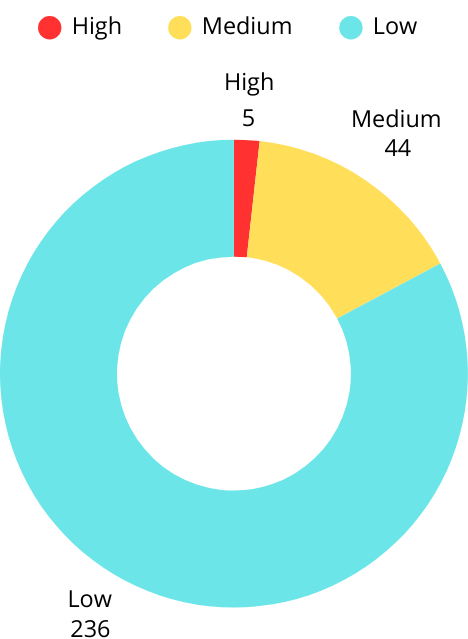
\includegraphics[width=0.5\textwidth]{assets/images-was/Total_Vulnerabilidades.png}
    \caption{Distribuição total de vulnerabilidades por severidade}
\end{figure}
\FloatBarrier

Abaixo, encontra-se um gráfico que apresenta o total de vulnerabilidades por site. Para um detalhamento mais específico sobre os quantitativos de vulnerabilidades de cada site, recomenda-se acessar os relatórios individuais de cada aplicação.

\begin{figure}[h!]
    \centering
    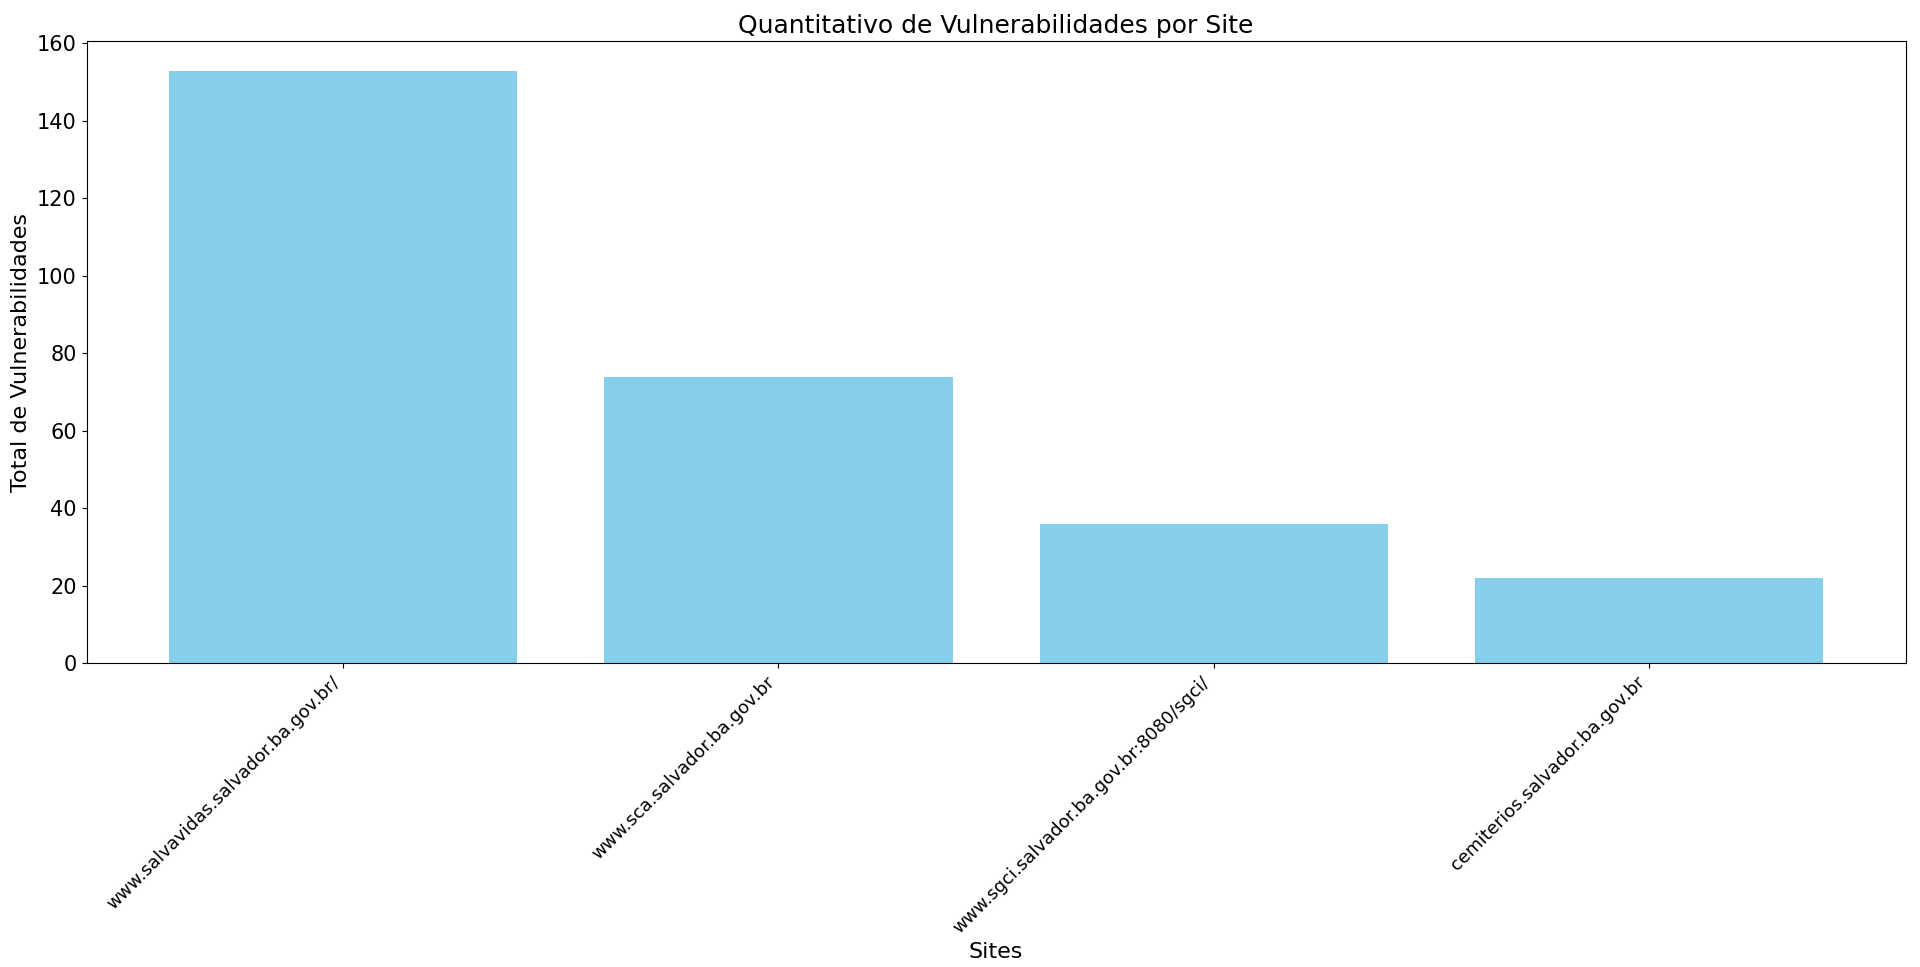
\includegraphics[width=1.0\textwidth]{assets/images-was/Vulnerabilidades_x_site.png}
    \caption{Total de vulnerabilidades por site}
\end{figure}
\FloatBarrier
As vulnerabilidades identificadas foram organizadas em seções e subseções, com o intuito de agrupá-las de acordo com sua afinidade e severidade. Cada seção aborda um conjunto específico de falhas de segurança, desde as relacionadas à configuração de segurança dos protocolos HTTP e TLS, até questões relacionadas à configuração inadequada do servidor e à exposição desnecessária de informações sensíveis. As subseções detalham vulnerabilidades em áreas como segurança de cookies e sessões, injeções de código, falhas de autenticação, entre outras. Essa estrutura facilita a análise, permitindo uma compreensão clara dos riscos e das recomendações de mitigação associadas a cada tipo de vulnerabilidade identificada.

%-------------- INÍCIO DA CATEGORIA Vulnerabilidades Relacionadas a Configurações de Segurança HTTP E TLS --------------
%-------------- INÍCIO DA CATEGORIA Vulnerabilidades Relacionadas a Configurações de Segurança HTTP E TLS --------------
\subsection{Vulnerabilidades Relacionadas a Configurações de Segurança HTTP E TLS}
Descrição não disponível.

%-------------- INÍCIO DA SUBCATEGORIA Informações de Cabeçalho --------------
\subsubsection{Informações de Cabeçalho}
Descrição não disponível.

\begin{enumerate}
%-------------- INÍCIO DA VULNERABILIDADE HTTP Header Information Disclosure --------------
\item \textbf{HTTP Header Information Disclosure}

                        \begin{figure}[h!]
                        \centering
                        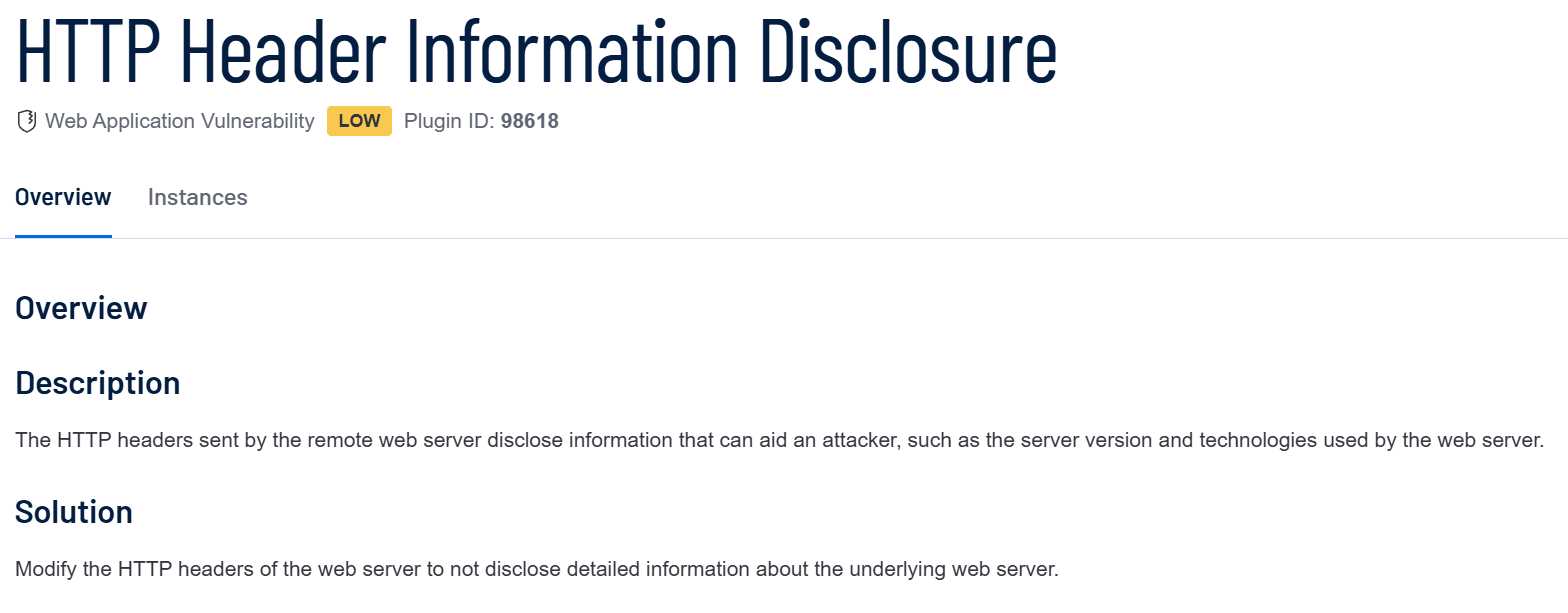
\includegraphics[width=0.8\textwidth]{assets/images-was/Vulnerabilidades Relacionadas a Configurações de Segurança HTTP E TLS/HTTP_header_Information_disclosure.png}
                        \end{figure}
                        \FloatBarrier
                        \textbf{Descrição:} A vulnerabilidade de divulgação de informações em cabeçalhos HTTP ocorre quando o servidor web remoto envia cabeçalhos que revelam detalhes sensíveis, como a versão do servidor e as tecnologias utilizadas. Essas informações podem ser exploradas por um atacante para identificar potenciais pontos fracos ou vulnerabilidades específicas, facilitando a execução de ataques direcionados.

    É crucial que as organizações implementem práticas de segurança, como a minimização das informações expostas nos cabeçalhos HTTP, para reduzir o risco de exploração. A configuração adequada do servidor pode mitigar a divulgação desnecessária de dados que possam ser utilizados para comprometer a segurança da aplicação.

\textbf{Solução:} Para mitigar essa vulnerabilidade, recomendamos a modificação dos cabeçalhos HTTP do servidor web para não divulgar informações detalhadas sobre o servidor subjacente. A desativação ou modificação de cabeçalhos como Server, X-Powered-By, X-AspNet-Version e outros cabeçalhos que revelam a versão ou a tecnologia do servidor é essencial.

\textbf{Total de URIs Afetadas:} 5

\textbf{Instâncias Afetadas:}
\begin{itemize}
    \item \url{http://gct.salvador.ba.gov.br}
    \item \url{https://www.credenciamento.salvador.ba.gov.br}
    \item \url{https://comunicacao.salvador.ba.gov.br}
    \item \url{http://agenciadenoticias.salvador.ba.gov.br}
    \item \url{http://dom.salvador.ba.gov.br}
\end{itemize}

%-------------- FIM DA VULNERABILIDADE HTTP Header Information Disclosure --------------
%-------------- INÍCIO DA VULNERABILIDADE Missing 'Cache-Control' Header --------------
\item \textbf{Missing 'Cache-Control' Header}

                        \begin{figure}[h!]
                        \centering
                        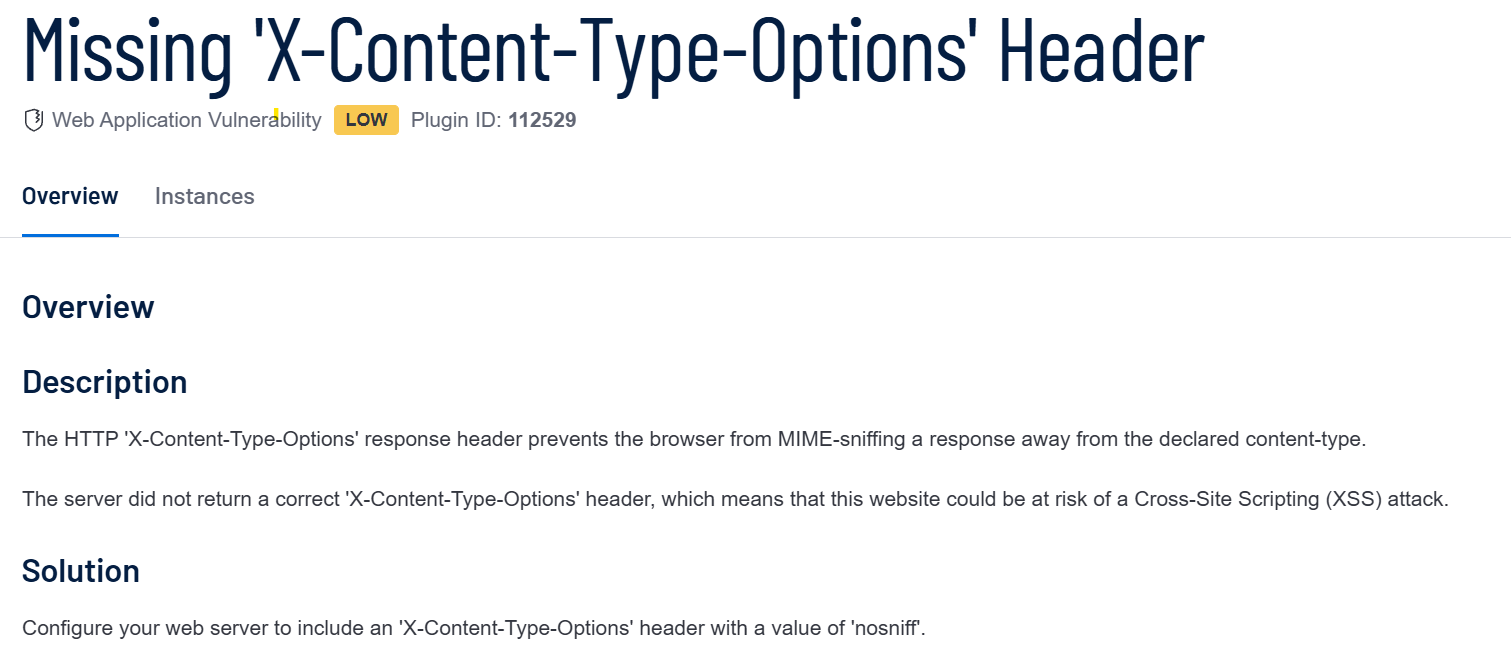
\includegraphics[width=0.8\textwidth]{assets/images-was/Vulnerabilidades Relacionadas a Configurações de Segurança HTTP E TLS/Missing 'X-Content-Type-Options' Header.png}
                        \end{figure}
                        \FloatBarrier
                        \textbf{Descrição:} A vulnerabilidade relacionada à ausência do cabeçalho X-Frame-Options ocorre quando o servidor web não envia o cabeçalho HTTP que define se a página pode ou não ser exibida em um frame ou iframe. Isso pode tornar o site vulnerável a ataques de clickjacking, onde um atacante manipula a interface do usuário para enganá-lo a clicar em algo diferente do que ele percebia, visando revelar informações confidenciais ou tomar controle do computador do usuário.

    A ausência do cabeçalho X-Frame-Options significa que o site pode ser incorporado em frames de outros sites, expondo os usuários a riscos de clickjacking. A implementação deste cabeçalho é uma medida importante para proteger os usuários contra esse tipo de ataque.

\textbf{Solução:} Para mitigar essa vulnerabilidade, recomenda-se configurar o servidor web para incluir o cabeçalho X-Frame-Options em todas as respostas HTTP. Isso pode ser feito configurando o servidor para permitir ou bloquear a exibição da página em frames, sendo recomendado o valor DENY ou SAMEORIGIN para evitar que o conteúdo seja incorporado em sites de terceiros.

\textbf{Total de URIs Afetadas:} 4

\textbf{Instâncias Afetadas:}
\begin{itemize}
    \item \url{https://comunicacao.salvador.ba.gov.br}
    \item \url{http://gct.salvador.ba.gov.br}
    \item \url{http://dom.salvador.ba.gov.br}
    \item \url{https://www.credenciamento.salvador.ba.gov.br}
\end{itemize}

%-------------- FIM DA VULNERABILIDADE Missing 'Cache-Control' Header --------------
%-------------- INÍCIO DA VULNERABILIDADE Missing Content Security Policy --------------
\item \textbf{Missing Content Security Policy}

                        \begin{figure}[h!]
                        \centering
                        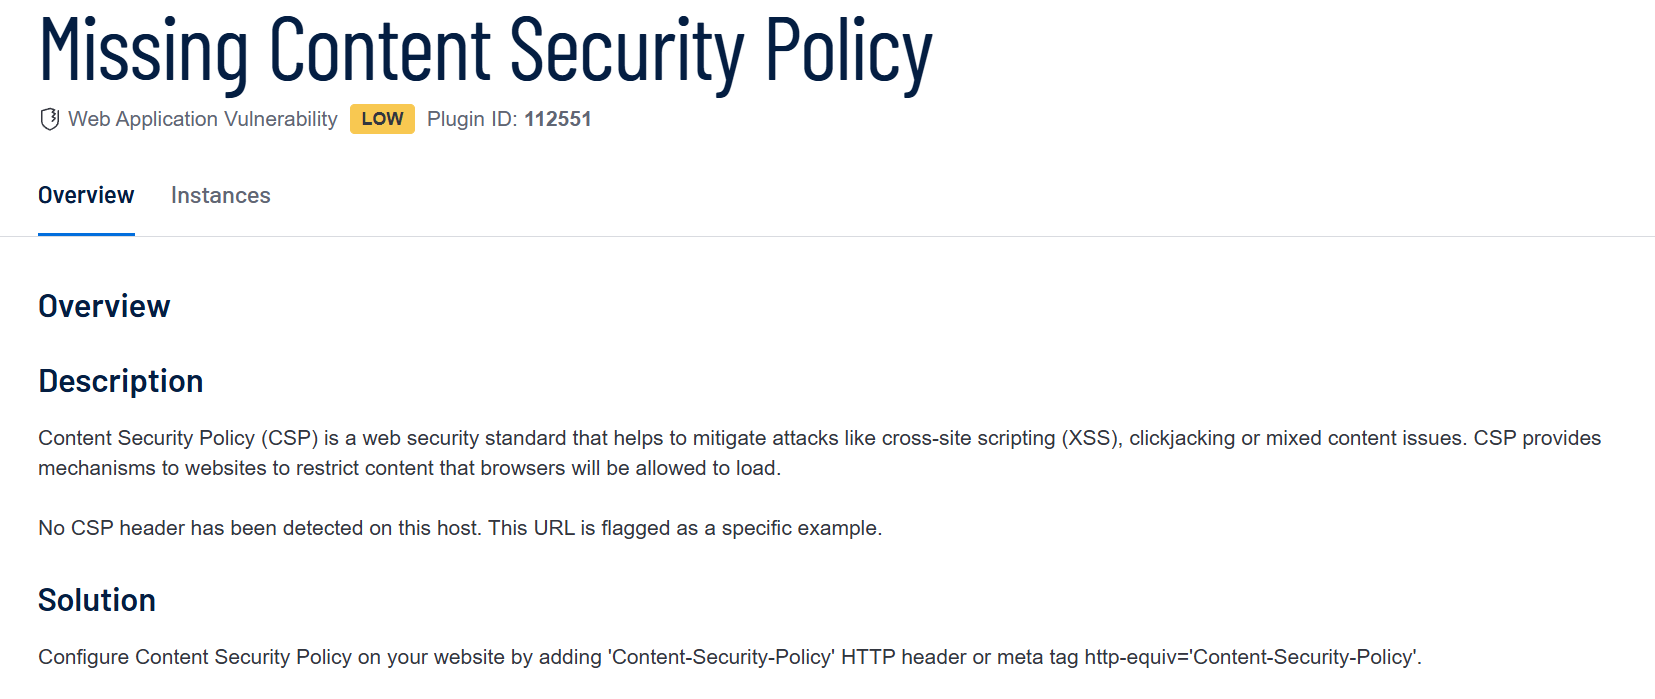
\includegraphics[width=0.8\textwidth]{assets/images-was/Vulnerabilidades Relacionadas a Configurações de Segurança HTTP E TLS/Missing Content Security Policy.png}
                        \end{figure}
                        \FloatBarrier
                        \textbf{Descrição:} A Política de Segurança de Conteúdo (CSP) é um padrão de segurança da web que ajuda a mitigar ataques como Cross-Site Scripting (XSS), clickjacking ou problemas de conteúdo misto. O CSP fornece mecanismos para que os sites restrinjam o conteúdo que os navegadores podem carregar.
 Nenhum cabeçalho CSP foi detectado neste host. Esta URL é sinalizada como um exemplo específico.

\textbf{Solução:} Configure a Política de Segurança de Conteúdo no seu site, adicionando o cabeçalho HTTP 'Content-Security-Policy' ou a tag meta http-equiv='Content-Security-Policy'.

\textbf{Total de URIs Afetadas:} 3

\textbf{Instâncias Afetadas:}
\begin{itemize}
    \item \url{http://gct.salvador.ba.gov.br}
    \item \url{http://dom.salvador.ba.gov.br}
    \item \url{https://www.credenciamento.salvador.ba.gov.br}
\end{itemize}

%-------------- FIM DA VULNERABILIDADE Missing Content Security Policy --------------
%-------------- INÍCIO DA VULNERABILIDADE Missing 'X-Content-Type-Options' Header --------------
\item \textbf{Missing 'X-Content-Type-Options' Header}

                        \begin{figure}[h!]
                        \centering
                        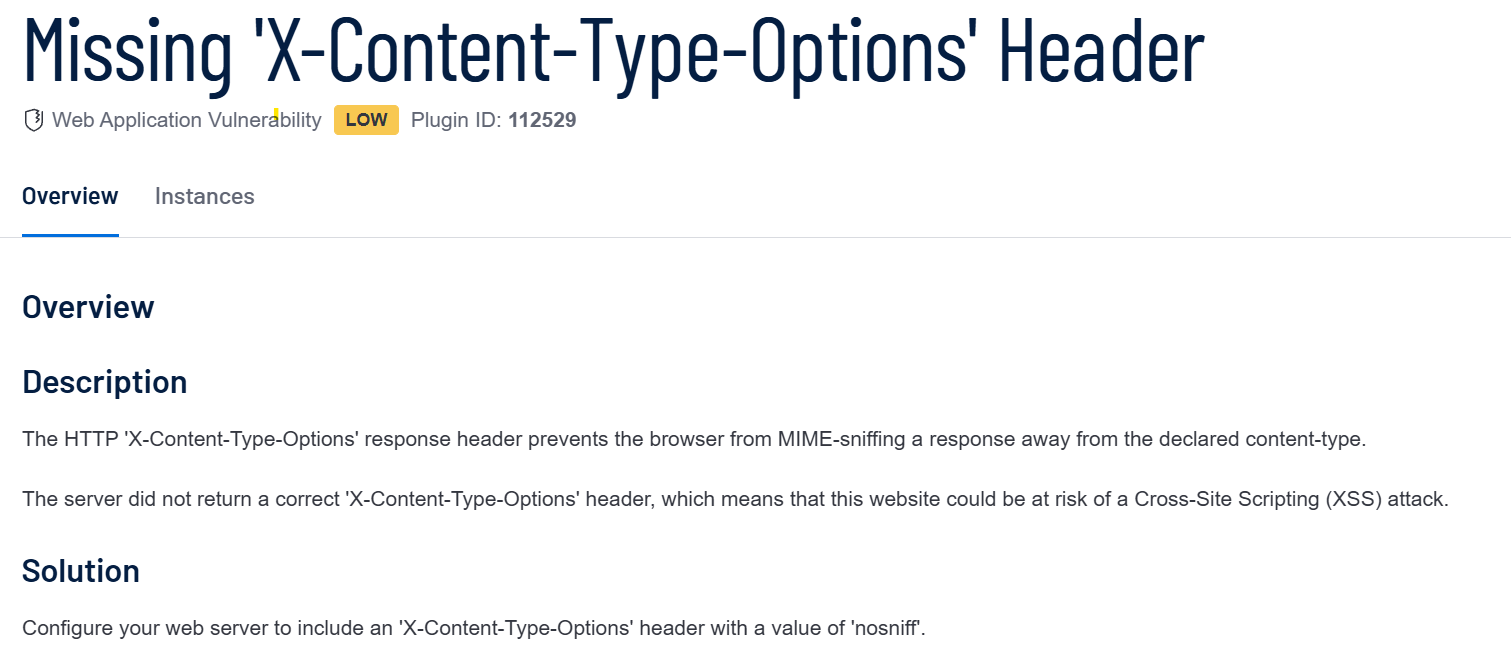
\includegraphics[width=0.8\textwidth]{assets/images-was/Vulnerabilidades Relacionadas a Configurações de Segurança HTTP E TLS/Missing 'X-Content-Type-Options' Header.png}
                        \end{figure}
                        \FloatBarrier
                        \textbf{Descrição:} A vulnerabilidade relacionada à ausência do cabeçalho X-Frame-Options ocorre quando o servidor web não envia o cabeçalho HTTP que define se a página pode ou não ser exibida em um frame ou iframe. Isso pode tornar o site vulnerável a ataques de clickjacking, onde um atacante manipula a interface do usuário para enganá-lo a clicar em algo diferente do que ele percebia, visando revelar informações confidenciais ou tomar controle do computador do usuário. A ausência do cabeçalho X-Frame-Options significa que o site pode ser incorporado em frames de outros sites, expondo os usuários a riscos de clickjacking. A implementação deste cabeçalho é uma medida importante para proteger os usuários contra esse tipo de ataque.

\textbf{Solução:} Para mitigar essa vulnerabilidade, recomenda-se configurar o servidor web para incluir o cabeçalho X-Frame-Options em todas as respostas HTTP. Isso pode ser feito configurando o servidor para permitir ou bloquear a exibição da página em frames, sendo recomendado o valor DENY ou SAMEORIGIN para evitar que o conteúdo seja incorporado em sites de terceiros.

\textbf{Total de URIs Afetadas:} 3

\textbf{Instâncias Afetadas:}
\begin{itemize}
    \item \url{http://gct.salvador.ba.gov.br}
    \item \url{http://dom.salvador.ba.gov.br}
    \item \url{https://www.credenciamento.salvador.ba.gov.br}
\end{itemize}

%-------------- FIM DA VULNERABILIDADE Missing 'X-Content-Type-Options' Header --------------
%-------------- INÍCIO DA VULNERABILIDADE Missing 'X-Frame-Options' Header --------------
\item \textbf{Missing 'X-Frame-Options' Header}

                        \begin{figure}[h!]
                        \centering
                        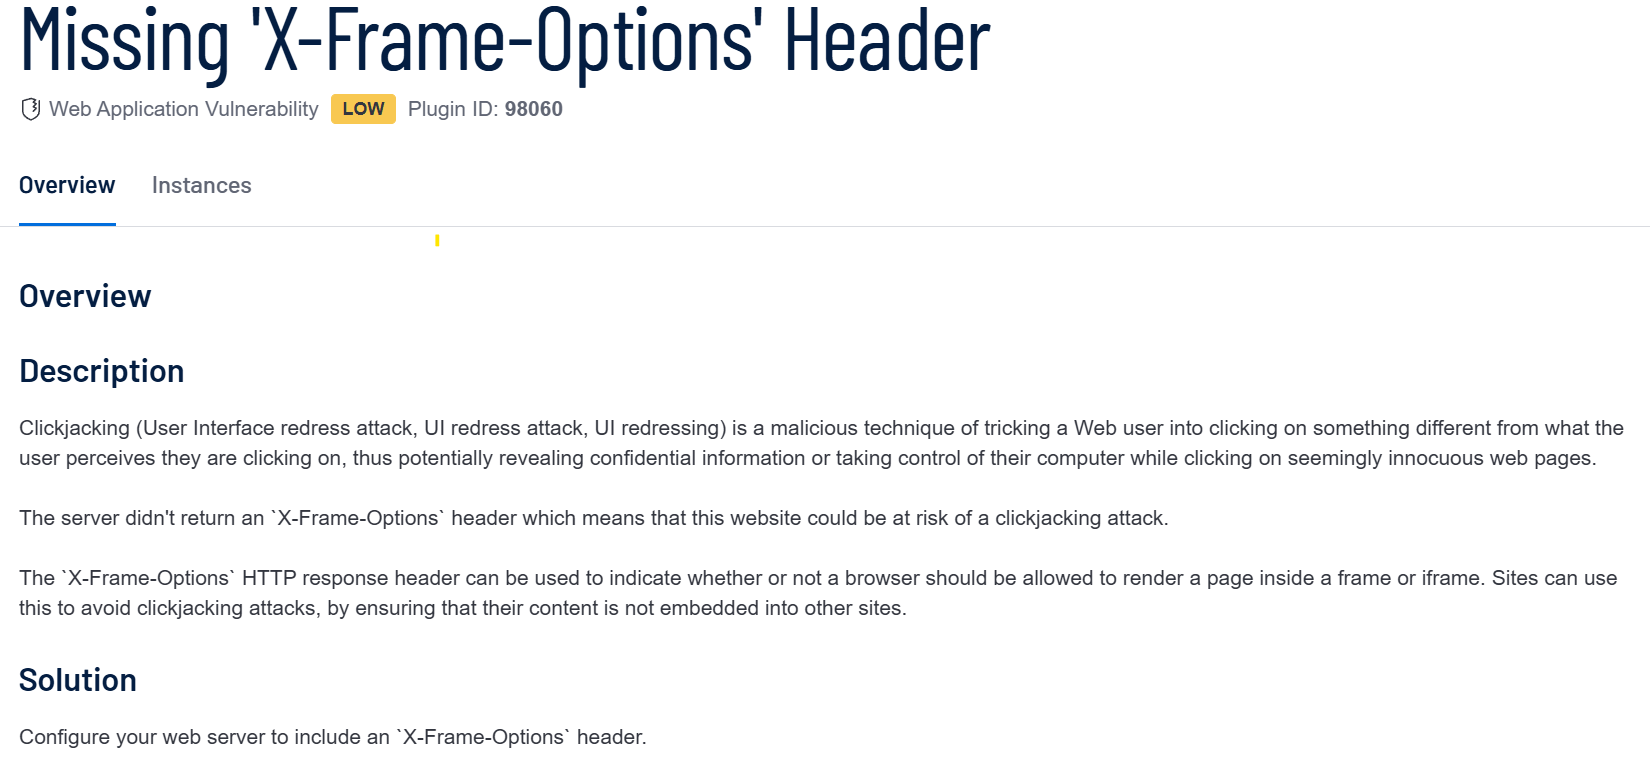
\includegraphics[width=0.8\textwidth]{assets/images-was/Vulnerabilidades Relacionadas a Configurações de Segurança HTTP E TLS/Missing 'X-Frame-Options' Header.png}
                        \end{figure}
                        \FloatBarrier
                        \textbf{Descrição:} A vulnerabilidade de ausência do cabeçalho X-Frame-Options ocorre quando o servidor web não retorna esse cabeçalho nas respostas HTTP. O cabeçalho X-Frame-Options é crucial para proteger os usuários contra ataques de clickjacking, um tipo de ataque onde o atacante engana o usuário a clicar em um elemento diferente do que ele percebe, frequentemente resultando na execução de ações não intencionais, como a revelação de informações confidenciais ou o controle do computador do usuário.

Sem a presença do cabeçalho X-Frame-Options, o conteúdo do site pode ser carregado em um frame ou iframe de outro site, o que facilita a exploração dessa vulnerabilidade. Isso ocorre porque um atacante pode embutir o site vulnerável em um iframe disfarçado, enganando o usuário a clicar em botões ou links que, na realidade, estão direcionados para outra ação maliciosa.

\textbf{Solução:} Para mitigar esse risco, recomenda-se configurar o servidor web para incluir o cabeçalho X-Frame-Options nas respostas HTTP. Esse cabeçalho pode ser configurado para bloquear a exibição da página em frames de outros sites, utilizando o valor DENY (proibindo completamente) ou SAMEORIGIN (permitindo apenas a exibição no mesmo domínio). Essa simples configuração ajuda a evitar que o conteúdo do site seja incorporado em páginas de terceiros, protegendo os usuários contra ataques de clickjacking.

\textbf{Total de URIs Afetadas:} 3

\textbf{Instâncias Afetadas:}
\begin{itemize}
    \item \url{https://comunicacao.salvador.ba.gov.br}
    \item \url{http://gct.salvador.ba.gov.br}
    \item \url{http://dom.salvador.ba.gov.br}
\end{itemize}

%-------------- FIM DA VULNERABILIDADE Missing 'X-Frame-Options' Header --------------
%-------------- INÍCIO DA VULNERABILIDADE Missing HTTP Strict Transport Security Policy --------------
\item \textbf{Missing HTTP Strict Transport Security Policy}

                        \begin{figure}[h!]
                        \centering
                        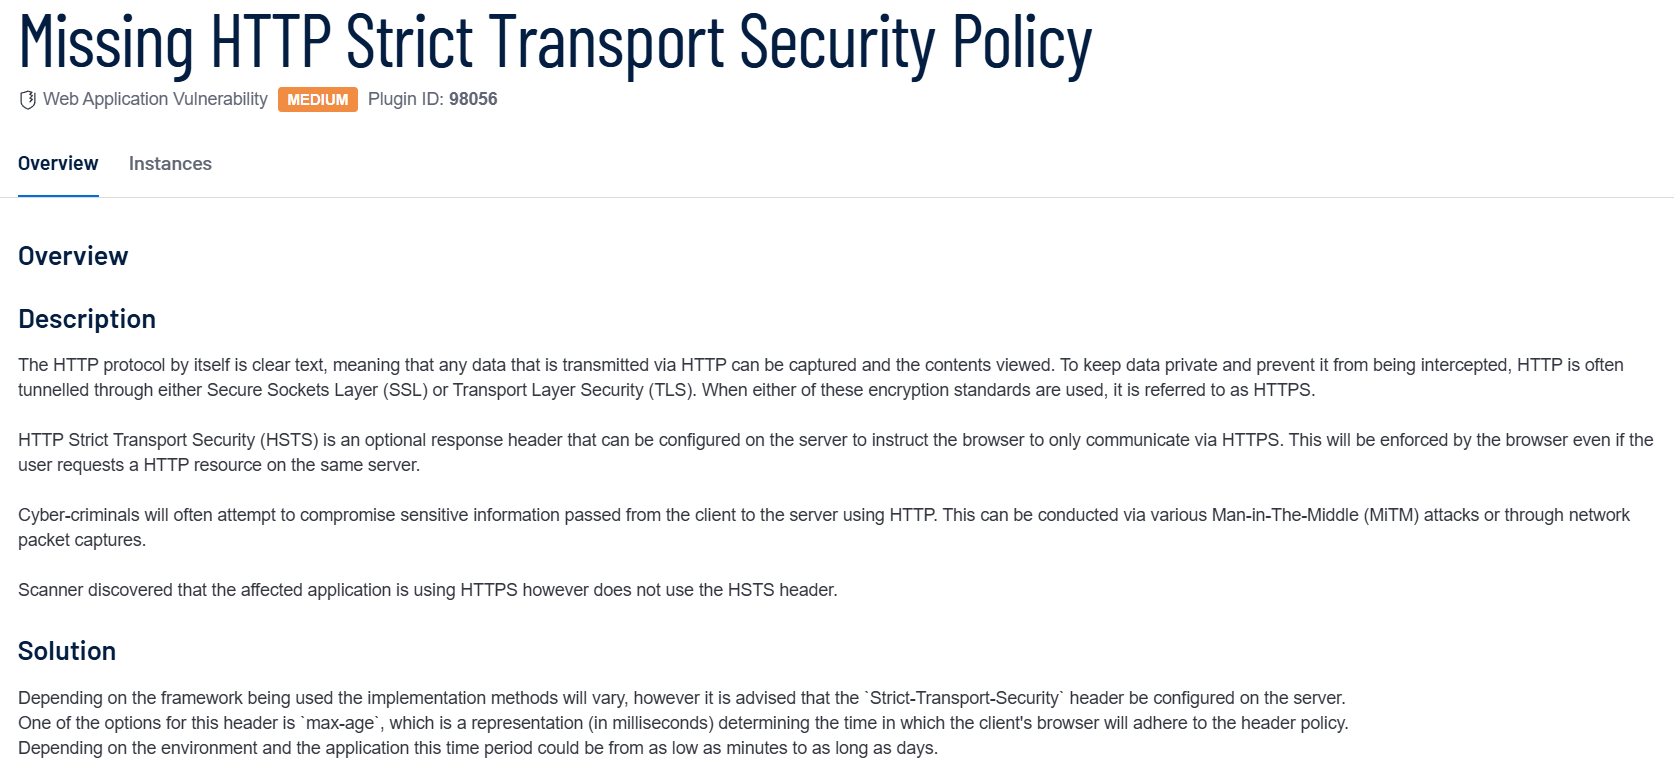
\includegraphics[width=0.8\textwidth]{assets/images-was/Vulnerabilidades Relacionadas a Configurações de Segurança HTTP E TLS/Missing HTTP Strict Transport Security Policy.png}
                        \end{figure}
                        \FloatBarrier
                        \textbf{Descrição:} O protocolo HTTP transmite dados em texto claro, o que significa que qualquer dado enviado via HTTP pode ser interceptado e visualizado. Para proteger a privacidade e evitar a interceptação de dados, o HTTP é frequentemente encapsulado através dos padrões de criptografia Secure Sockets Layer (SSL) ou Transport Layer Security (TLS), resultando no uso de HTTPS.

O HTTP Strict Transport Security (HSTS) é um cabeçalho de resposta opcional que pode ser configurado no servidor para instruir o navegador a se comunicar exclusivamente via HTTPS. Essa política será forçada pelo navegador, mesmo que o usuário tente acessar um recurso HTTP na mesma origem. O HSTS ajuda a proteger contra ataques de downgrade, em que um atacante pode tentar forçar uma conexão insegura em vez de usar a versão segura HTTPS.

Criminosos cibernéticos costumam tentar comprometer informações sensíveis transmitidas entre o cliente e o servidor via HTTP, utilizando técnicas como ataques Man-in-The-Middle (MiTM) ou capturas de pacotes de rede. Embora a aplicação afetada utilize HTTPS, ela não está utilizando o cabeçalho HSTS, o que a deixa vulnerável a esse tipo de ataque.

\textbf{Solução:} Para mitigar esse risco, é altamente recomendado configurar o cabeçalho Strict-Transport-Security no servidor. Esse cabeçalho instrui os navegadores a forçar o uso do HTTPS e a garantir que, mesmo que o usuário tente acessar uma versão HTTP de um recurso, a comunicação será automaticamente redirecionada para HTTPS. Uma das opções para configurar o cabeçalho é o parâmetro max-age, que define o tempo (em segundos) pelo qual o navegador deve seguir a política de HSTS. O período pode variar conforme o ambiente e os requisitos da aplicação, podendo ser de alguns minutos até vários dias.

\textbf{Total de URIs Afetadas:} 2

\textbf{Instâncias Afetadas:}
\begin{itemize}
    \item \url{http://dom.salvador.ba.gov.br}
    \item \url{https://www.credenciamento.salvador.ba.gov.br}
\end{itemize}

%-------------- FIM DA VULNERABILIDADE Missing HTTP Strict Transport Security Policy --------------
%-------------- INÍCIO DA VULNERABILIDADE Missing 'Content-Type' Header --------------
\item \textbf{Missing 'Content-Type' Header}

                        \begin{figure}[h!]
                        \centering
                        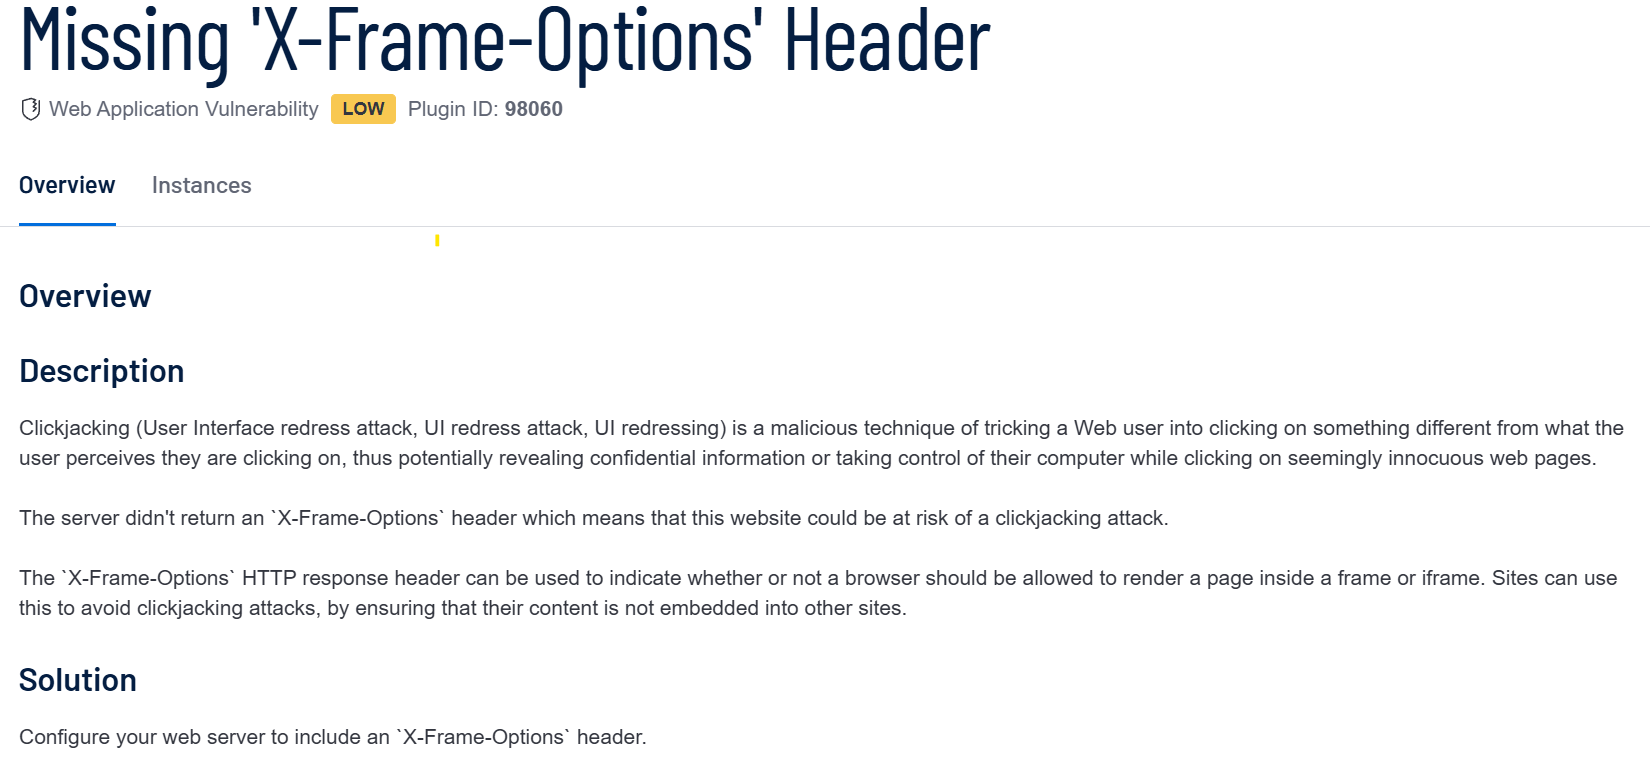
\includegraphics[width=0.8\textwidth]{assets/images-was/Vulnerabilidades Relacionadas a Configurações de Segurança HTTP E TLS/Missing 'X-Frame-Options' Header.png}
                        \end{figure}
                        \FloatBarrier
                        \textbf{Descrição:} A vulnerabilidade de ausência do cabeçalho X-Frame-Options ocorre quando o servidor web não retorna esse cabeçalho nas respostas HTTP. O cabeçalho X-Frame-Options é crucial para proteger os usuários contra ataques de clickjacking, um tipo de ataque onde o atacante engana o usuário a clicar em um elemento diferente do que ele percebe, frequentemente resultando na execução de ações não intencionais, como a revelação de informações confidenciais ou o controle do computador do usuário.

    Sem a presença do cabeçalho X-Frame-Options, o conteúdo do site pode ser carregado em um frame ou iframe de outro site, o que facilita a exploração dessa vulnerabilidade. Isso ocorre porque um atacante pode embutir o site vulnerável em um iframe disfarçado, enganando o usuário a clicar em botões ou links que, na realidade, estão direcionados para outra ação maliciosa.

\textbf{Solução:} Para mitigar esse risco, recomenda-se configurar o servidor web para incluir o cabeçalho X-Frame-Options nas respostas HTTP. Esse cabeçalho pode ser configurado para bloquear a exibição da página em frames de outros sites, utilizando o valor DENY (proibindo completamente) ou SAMEORIGIN (permitindo apenas a exibição no mesmo domínio). Essa simples configuração ajuda a evitar que o conteúdo do site seja incorporado em páginas de terceiros, protegendo os usuários contra ataques de clickjacking.

\textbf{Total de URIs Afetadas:} 1

\textbf{Instâncias Afetadas:}
\begin{itemize}
    \item \url{https://www.credenciamento.salvador.ba.gov.br}
\end{itemize}

%-------------- FIM DA VULNERABILIDADE Missing 'Content-Type' Header --------------
%-------------- INÍCIO DA VULNERABILIDADE Mixed Resource Detection --------------
\item \textbf{Mixed Resource Detection}

                        \begin{figure}[h!]
                        \centering
                        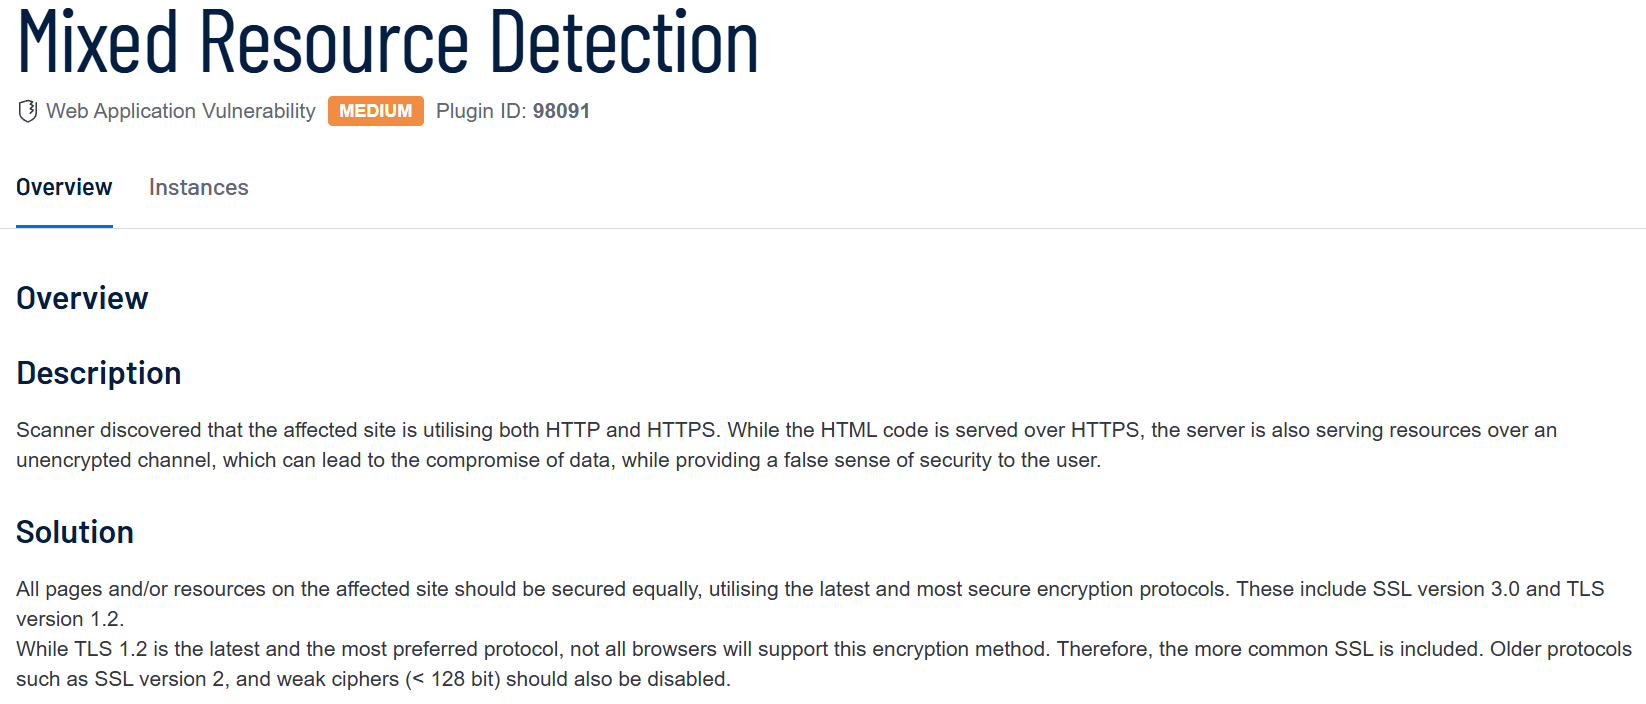
\includegraphics[width=0.8\textwidth]{assets/images-was/Vulnerabilidades Relacionadas a Configurações de Segurança HTTP E TLS/Mixed Resource Detection}
                        \end{figure}
                        \FloatBarrier
                        \textbf{Descrição:} O scanner descobriu que o site afetado está utilizando tanto HTTP quanto HTTPS. Embora o código HTML seja servido via HTTPS, o servidor também está fornecendo recursos por um canal não criptografado, o que pode comprometer os dados, ao mesmo tempo que oferece uma falsa sensação de segurança ao usuário.


\textbf{Solução:} Todas as páginas e/ou recursos no site afetado devem ser igualmente protegidos, utilizando os protocolos de criptografia mais seguros e recentes, como TLS 1.2 e TLS 1.3.

\textbf{Total de URIs Afetadas:} 1

\textbf{Instâncias Afetadas:}
\begin{itemize}
    \item \url{https://www.credenciamento.salvador.ba.gov.br}
\end{itemize}

%-------------- FIM DA VULNERABILIDADE Mixed Resource Detection --------------
%-------------- INÍCIO DA VULNERABILIDADE Permissive HTTP Strict Transport Security Policy Detected --------------
\item \textbf{Permissive HTTP Strict Transport Security Policy Detected}

                        \begin{figure}[h!]
                        \centering
                        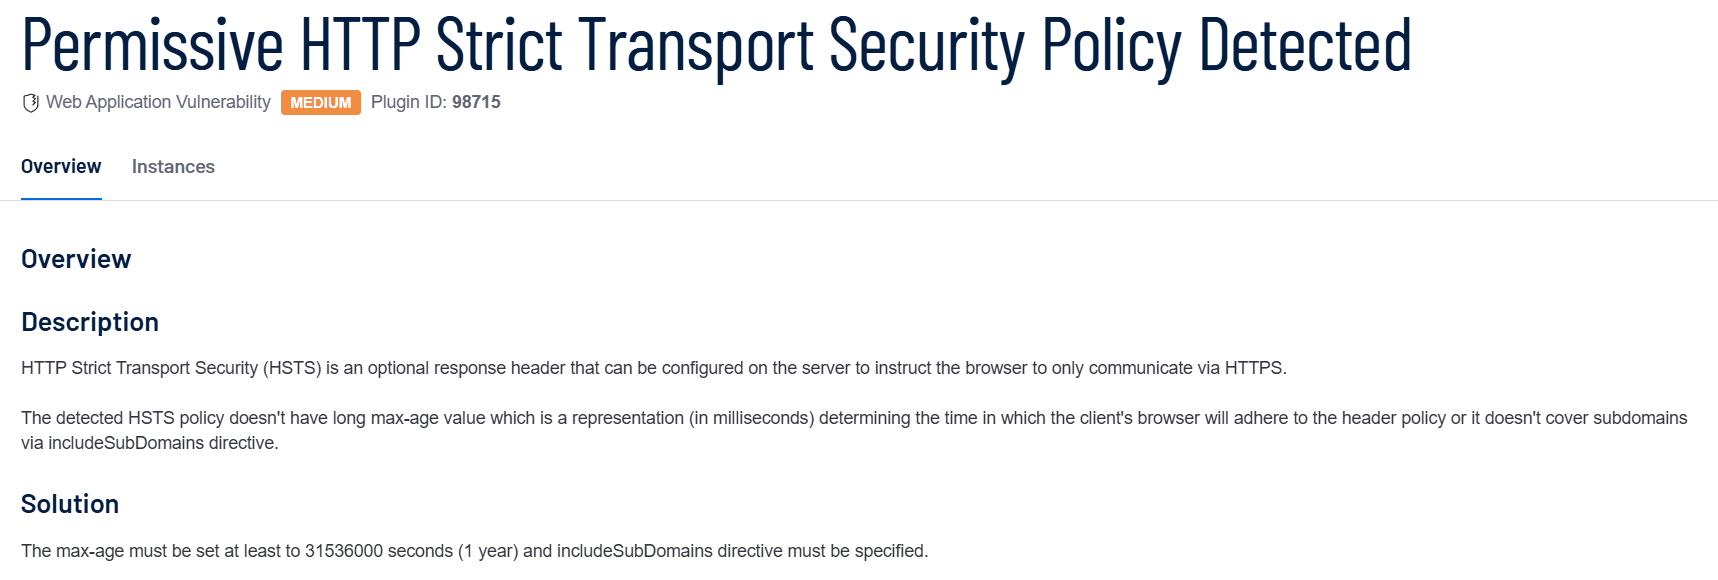
\includegraphics[width=0.8\textwidth]{assets/images-was/Vulnerabilidades Relacionadas a Configurações de Segurança HTTP E TLS/Permissive HTTP Strict Transport Security Policy Detected.png}
                        \end{figure}
                        \FloatBarrier
                        \textbf{Descrição:} O HTTP Strict Transport Security (HSTS) é um cabeçalho de resposta opcional que pode ser configurado no servidor para instruir o navegador a se comunicar exclusivamente via HTTPS. Ao ser configurado corretamente, o HSTS ajuda a proteger os usuários contra ataques de downgrade e interceptação de dados. No entanto, foi detectado que a política HSTS configurada para o servidor não possui um valor suficientemente longo para o parâmetro max-age ou não cobre subdomínios por meio da diretiva includeSubDomains.

\textbf{Solução:} Para melhorar a segurança e evitar que a política HSTS seja permissiva demais, é recomendado ajustar o parâmetro max-age para um valor de, pelo menos, 31536000 segundos (1 ano). Além disso, a diretiva includeSubDomains deve ser especificada para garantir que todos os subdomínios sejam protegidos pela mesma política HSTS.

\textbf{Total de URIs Afetadas:} 1

\textbf{Instâncias Afetadas:}
\begin{itemize}
    \item \url{https://comunicacao.salvador.ba.gov.br}
\end{itemize}

%-------------- FIM DA VULNERABILIDADE Permissive HTTP Strict Transport Security Policy Detected --------------
\end{enumerate}
%-------------- FIM DA SUBCATEGORIA Informações de Cabeçalho --------------
%-------------- INÍCIO DA SUBCATEGORIA Protocolos e Cifragem --------------
\subsubsection{Protocolos e Cifragem}
Esta subseção aborda a vulnerabilidade de protocolos e mecanismos de cifragem inadequados ou desatualizados em implementações TLS/SSL. Configurações fracas de criptografia podem permitir a interceptação de dados sensíveis, comprometendo a confidencialidade e integridade das informações.

\begin{enumerate}
%-------------- INÍCIO DA VULNERABILIDADE SSL/TLS Weak Cipher Suites Supported --------------
\item \textbf{SSL/TLS Weak Cipher Suites Supported}

                        \begin{figure}[h!]
                        \centering
                        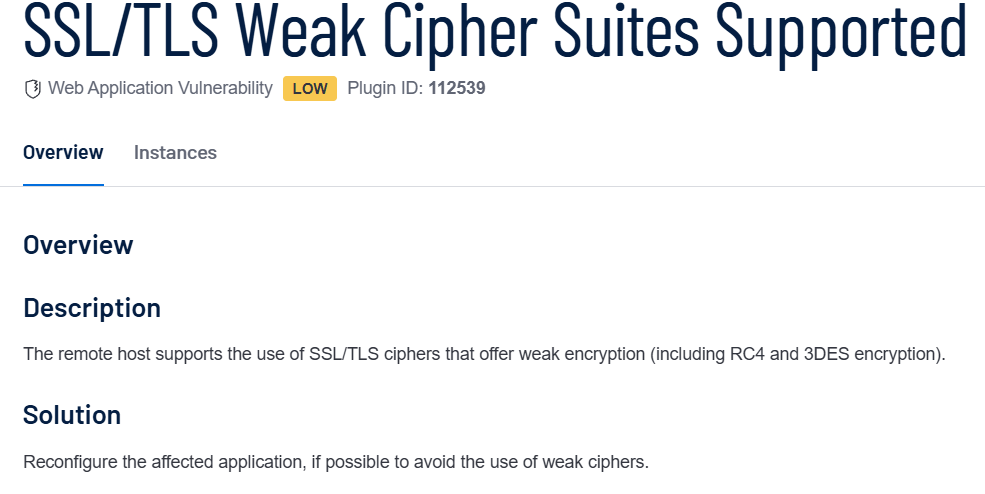
\includegraphics[width=0.8\textwidth]{assets/images-was/Protocolos e Cifragem/SSL-TLS Weak Cipher Suites Supported.png}
                        \end{figure}
                        \FloatBarrier
                        \textbf{Descrição:} O servidor remoto suporta o uso de conjuntos de cifras (cipher suites) de SSL/TLS que oferecem criptografia insegura, incluindo suites de exportação e cifras com menos de 128 bits. Esses conjuntos de cifras são considerados inseguros porque proporcionam um nível de proteção inadequado, tornando mais fácil para um atacante decifrar os dados transmitidos.

    Conjuntos de cifras com menos de 128 bits de força não oferecem uma barreira suficiente contra ataques de força bruta e outros métodos de comprometimento de dados. O suporte a essas cifras pode expor a comunicação a riscos significativos, incluindo a interceptação de dados sensíveis e a perda da integridade da transmissão.

\textbf{Solução:} Recomenda-se reconfigurar a aplicação ou servidor afetado para desabilitar o suporte a conjuntos de cifras fracas. As cifras mais seguras, como AES (Advanced Encryption Standard) em modos de operação modernos (por exemplo, GCM), devem ser priorizadas. Além disso, a configuração do servidor deve ser revisada para garantir o suporte a protocolos e algoritmos de criptografia que estejam de acordo com as melhores práticas de segurança, como TLS 1.2 ou TLS 1.3, que oferecem melhorias significativas em segurança e desempenho.

\textbf{Total de URIs Afetadas:} 5

\textbf{Instâncias Afetadas:}
\begin{itemize}
    \item \url{http://gct.salvador.ba.gov.br}
    \item \url{https://www.credenciamento.salvador.ba.gov.br}
    \item \url{https://comunicacao.salvador.ba.gov.br}
    \item \url{http://agenciadenoticias.salvador.ba.gov.br}
    \item \url{http://dom.salvador.ba.gov.br}
\end{itemize}

%-------------- FIM DA VULNERABILIDADE SSL/TLS Weak Cipher Suites Supported --------------
%-------------- INÍCIO DA VULNERABILIDADE SSL/TLS Forward Secrecy Cipher Suites Not Supported --------------
\item \textbf{SSL/TLS Forward Secrecy Cipher Suites Not Supported}

                        \begin{figure}[h!]
                        \centering
                        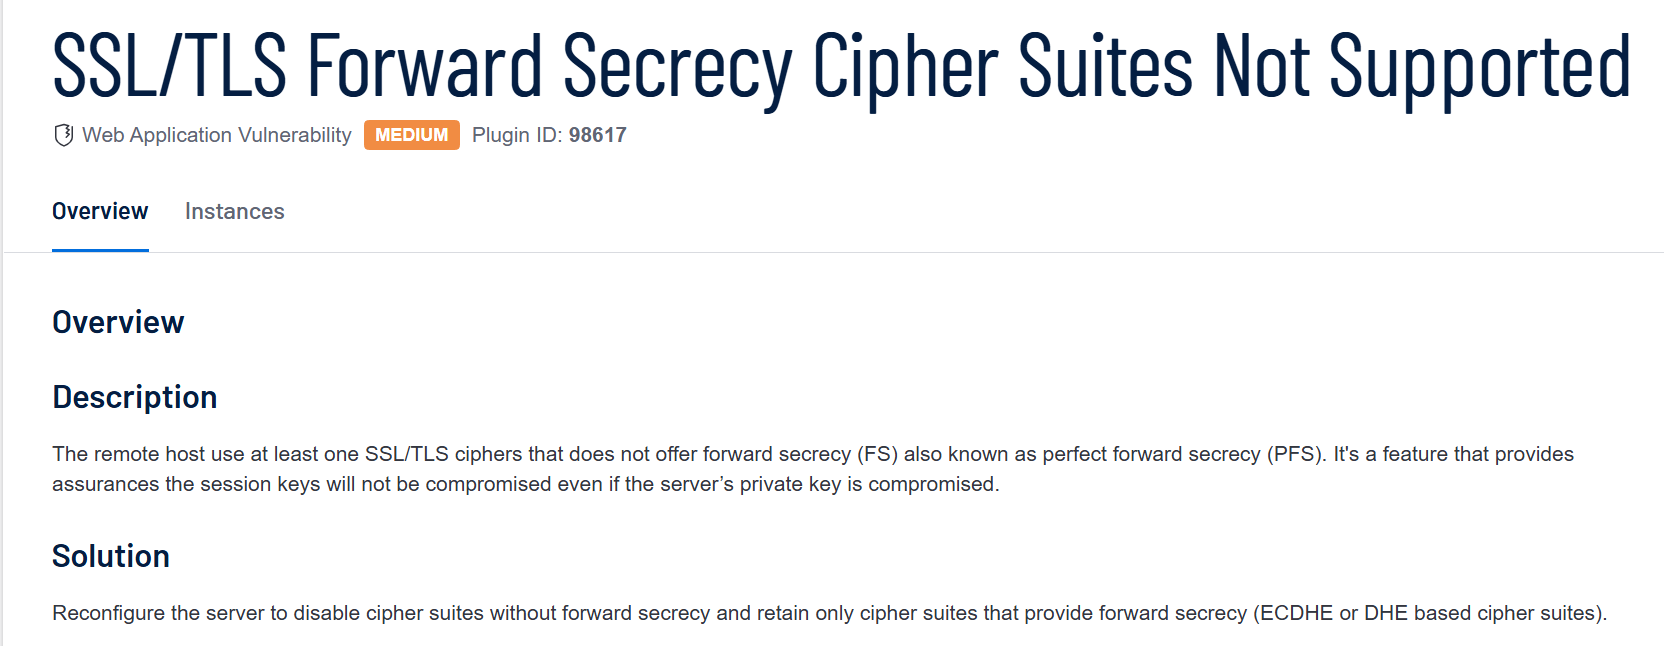
\includegraphics[width=0.8\textwidth]{assets/images-was/Protocolos e Cifragem/SSL-TLS Forward Secrecy Cipher Suites Not Supported}
                        \end{figure}
                        \FloatBarrier
                        \textbf{Descrição:} O host remoto utiliza pelo menos uma cifra SSL/TLS que não oferece segredo perfeito (FS), também conhecido como segredo perfeito de avanço (PFS). Essa é uma característica que garante que as chaves de sessão não serão comprometidas mesmo que a chave privada do servidor seja comprometida.


\textbf{Solução:} Reconfigure o servidor para desabilitar as cifras sem segredo perfeito e mantenha apenas as cifras que oferecem segredo perfeito (cifras baseadas em ECDHE ou DHE).

\textbf{Total de URIs Afetadas:} 5

\textbf{Instâncias Afetadas:}
\begin{itemize}
    \item \url{http://gct.salvador.ba.gov.br}
    \item \url{https://www.credenciamento.salvador.ba.gov.br}
    \item \url{https://comunicacao.salvador.ba.gov.br}
    \item \url{http://agenciadenoticias.salvador.ba.gov.br}
    \item \url{http://dom.salvador.ba.gov.br}
\end{itemize}

%-------------- FIM DA VULNERABILIDADE SSL/TLS Forward Secrecy Cipher Suites Not Supported --------------
%-------------- INÍCIO DA VULNERABILIDADE SSL/TLS Certificate Expired --------------
\item \textbf{SSL/TLS Certificate Expired}

                        \begin{figure}[h!]
                        \centering
                        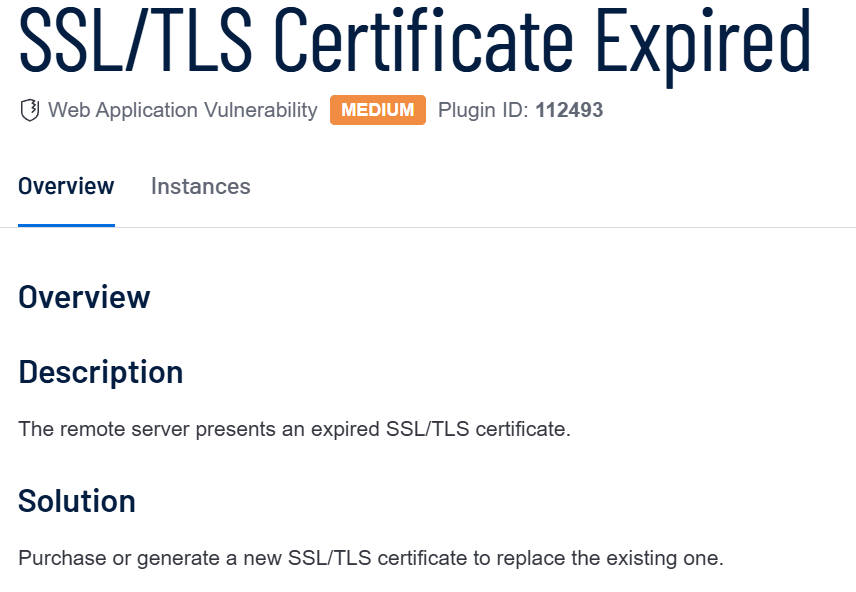
\includegraphics[width=0.8\textwidth]{assets/images-was/Protocolos e Cifragem/SSL-TLS Certificate Expired.png}
                        \end{figure}
                        \FloatBarrier
                        \textbf{Descrição:} O servidor remoto apresenta um certificado SSL/TLS no qual o Common Name (CN) e o Subject Alternative Name (SAN) não correspondem ao nome de host do servidor. O Common Name e o Subject Alternative Name são campos no certificado que devem refletir os domínios e subdomínios que o certificado protege. Quando esses campos não coincidem com o nome de host do servidor, pode ocorrer um erro de validação do certificado, levando os navegadores e clientes a desconfiarem da identidade do servidor.

    Esse tipo de mismatch pode ocorrer devido a um erro na emissão do certificado, em que os nomes registrados não correspondem ao nome real do servidor, comprometendo a confiança e a integridade da conexão. Além disso, pode ser um indicativo de que o servidor está sendo mal configurado ou de um possível ataque de man-in-the-middle.

\textbf{Solução:} Para corrigir essa vulnerabilidade, é necessário adquirir ou gerar um novo certificado SSL/TLS para substituir o atual, priorizando o certificado TLS 1.2 e superior. O novo certificado deve ser configurado corretamente no servidor para garantir que todas as conexões sejam criptografadas com um certificado válido. Além disso, é importante configurar alertas ou monitoramento para garantir que o certificado seja renovado antes de sua expiração no futuro.

\textbf{Total de URIs Afetadas:} 2

\textbf{Instâncias Afetadas:}
\begin{itemize}
    \item \url{http://gct.salvador.ba.gov.br}
    \item \url{http://dom.salvador.ba.gov.br}
\end{itemize}

%-------------- FIM DA VULNERABILIDADE SSL/TLS Certificate Expired --------------
%-------------- INÍCIO DA VULNERABILIDADE TLS 1.0 Weak Protocol --------------
\item \textbf{TLS 1.0 Weak Protocol}

                        \begin{figure}[h!]
                        \centering
                        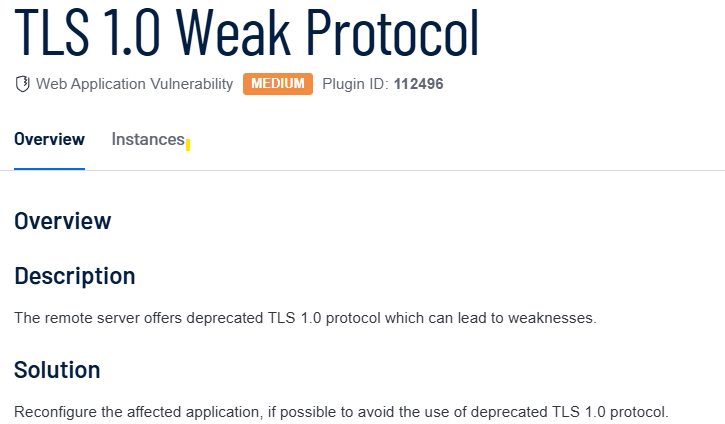
\includegraphics[width=0.8\textwidth]{assets/images-was/Protocolos e Cifragem/TLS 1.0 Weak Protocol.png}
                        \end{figure}
                        \FloatBarrier
                        \textbf{Descrição:} O servidor remoto suporta o uso de conjuntos de cifras (cipher suites) de SSL/TLS que oferecem criptografia fraca, como RC4 e 3DES. Esses algoritmos de criptografia estão obsoletos e possuem vulnerabilidades conhecidas que podem ser exploradas por atacantes para comprometer a confidencialidade e a integridade dos dados transmitidos.

    O uso de cifras fracas, como RC4, que está suscetível a ataques de viés de chave, e 3DES, que é vulnerável a ataques de colisão devido ao seu tamanho de chave efetivo de 112 bits, enfraquece a segurança da comunicação entre o cliente e o servidor. Isso pode resultar em ataques de interceptação e roubo de dados, comprometendo a segurança da aplicação e seus usuários.

\textbf{Solução:} Para mitigar essa vulnerabilidade, recomenda-se reconfigurar a aplicação ou o servidor afetado para desabilitar o uso do protocolo TLS 1.0. Em vez disso, deve-se usar versões mais seguras do protocolo, como TLS 1.2 ou TLS 1.3, que oferecem melhorias significativas em termos de segurança e desempenho. A atualização para essas versões mais recentes ajuda a proteger a comunicação de ameaças conhecidas e garante uma experiência mais segura para os usuários.

\textbf{Total de URIs Afetadas:} 2

\textbf{Instâncias Afetadas:}
\begin{itemize}
    \item \url{http://agenciadenoticias.salvador.ba.gov.br}
    \item \url{http://dom.salvador.ba.gov.br}
\end{itemize}

%-------------- FIM DA VULNERABILIDADE TLS 1.0 Weak Protocol --------------
%-------------- INÍCIO DA VULNERABILIDADE TLS 1.1 Weak Protocol --------------
\item \textbf{TLS 1.1 Weak Protocol}

                        \begin{figure}[h!]
                        \centering
                        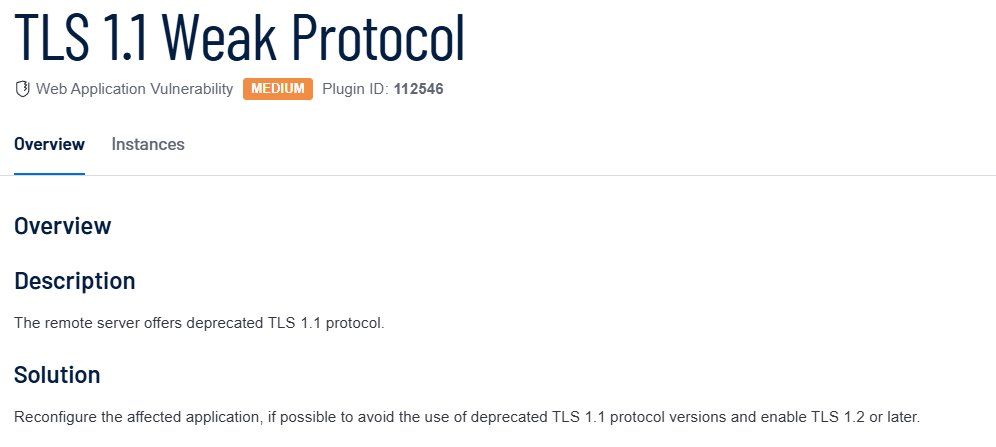
\includegraphics[width=0.8\textwidth]{assets/images-was/Protocolos e Cifragem/TLS 1.1 Weak Protocol.png}
                        \end{figure}
                        \FloatBarrier
                        \textbf{Descrição:} O protocolo TLS 1.0, introduzido em 1999, foi um importante avanço para a segurança da comunicação na web, mas é atualmente considerado obsoleto devido a diversas vulnerabilidades que podem ser exploradas por atacantes. O uso do TLS 1.0 apresenta riscos de segurança, como a possibilidade de ataques de downgrade e a exploração de algoritmos de criptografia mais fracos. Isso pode resultar na exposição de dados sensíveis transmitidos entre o cliente e o servidor.

    Manter o suporte a protocolos depreciados como o TLS 1.0 pode enfraquecer a postura de segurança da aplicação e deixar os usuários vulneráveis a ataques cibernéticos que exploram essas falhas conhecidas.

\textbf{Solução:} Recomenda-se a reconfiguração da aplicação afetada para desabilitar o uso do protocolo TLS 1.0. Deve-se optar pelo uso de TLS 1.2 ou, preferencialmente, TLS 1.3, que proporcionam níveis de segurança substancialmente superiores, com mecanismos de criptografia mais robustos e menor susceptibilidade a vulnerabilidades exploradas em versões anteriores.

\textbf{Total de URIs Afetadas:} 2

\textbf{Instâncias Afetadas:}
\begin{itemize}
    \item \url{http://agenciadenoticias.salvador.ba.gov.br}
    \item \url{http://dom.salvador.ba.gov.br}
\end{itemize}

%-------------- FIM DA VULNERABILIDADE TLS 1.1 Weak Protocol --------------
\end{enumerate}
%-------------- FIM DA SUBCATEGORIA Protocolos e Cifragem --------------
%-------------- FIM DA CATEGORIA Vulnerabilidades Relacionadas a Configurações de Segurança HTTP E TLS --------------
%-------------- INÍCIO DA CATEGORIA Vulnerabilidades Relacionadas a Configurações e Exposição de Informações --------------
\subsection{Vulnerabilidades Relacionadas a Configurações e Exposição de Informações}
Descrição não disponível.

%-------------- INÍCIO DA SUBCATEGORIA Configurações do Servidor --------------
\subsubsection{Configurações do Servidor}
Descrição não disponível.

\begin{enumerate}
%-------------- INÍCIO DA VULNERABILIDADE Access Restriction Bypass Via Origin Spoof --------------
\item \textbf{Access Restriction Bypass Via Origin Spoof}

                        \begin{figure}[h!]
                        \centering
                        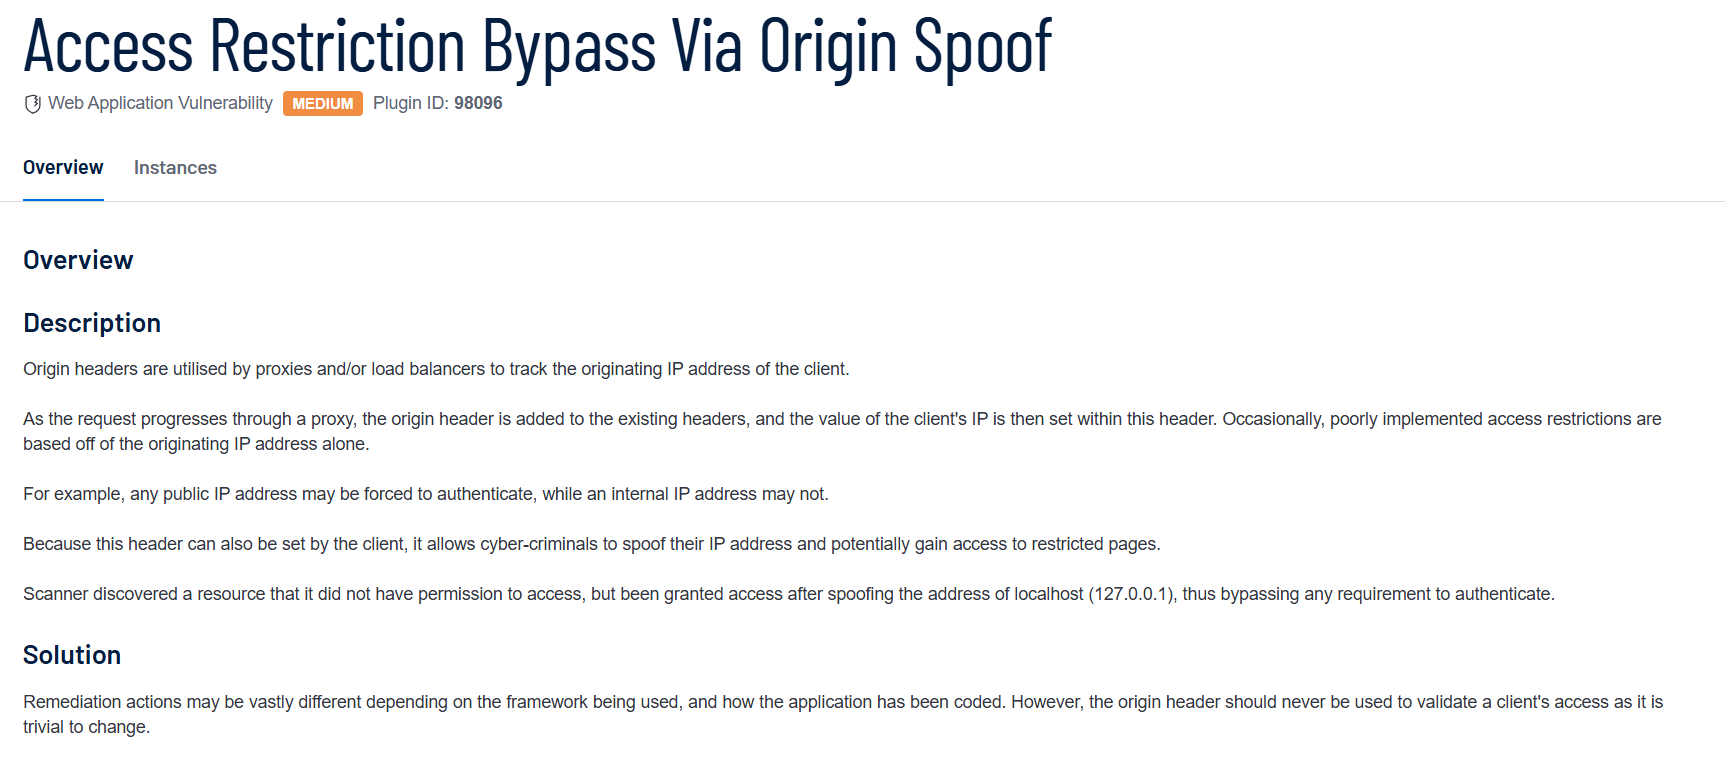
\includegraphics[width=0.8\textwidth]{assets/images-was/Vulnerabilidades Relacionadas a Configurações e Exposição de Informações/Configurações do Servidor/Access Restriction Bypass Via Origin Spoof.png}
                        \end{figure}
                        \FloatBarrier
                        \textbf{Descrição:} Os cabeçalhos de origem (Origin headers) são utilizados por proxies e/ou balanceadores de carga para rastrear o endereço IP de origem do cliente. À medida que a requisição progride por um proxy, o cabeçalho de origem é adicionado aos cabeçalhos existentes, e o valor do IP do cliente é definido neste cabeçalho. Em algumas ocasiões, restrições de acesso mal implementadas são baseadas exclusivamente no endereço IP de origem. Por exemplo, qualquer endereço IP público pode ser obrigado a autenticar, enquanto um endereço IP interno pode não ser. Como este cabeçalho também pode ser configurado pelo cliente, ele permite que criminosos cibernéticos falsifiquem seu endereço IP e, potencialmente, obtenham acesso a páginas restritas. O scanner descobriu um recurso ao qual não tinha permissão para acessar, mas conseguiu acesso após falsificar o endereço de localhost (127.0.0.1), contornando assim a exigência de autenticação.

\textbf{Solução:} As ações corretivas podem variar amplamente dependendo do framework utilizado e de como a aplicação foi codificada. No entanto, o cabeçalho de origem nunca deve ser usado para validar o acesso de um cliente, pois ele é trivialmente modificável.

\textbf{Total de URIs Afetadas:} 2

\textbf{Instâncias Afetadas:}
\begin{itemize}
    \item \url{http://gct.salvador.ba.gov.br}
    \item \url{http://dom.salvador.ba.gov.br}
\end{itemize}

%-------------- FIM DA VULNERABILIDADE Access Restriction Bypass Via Origin Spoof --------------
\end{enumerate}
%-------------- FIM DA SUBCATEGORIA Configurações do Servidor --------------
%-------------- INÍCIO DA SUBCATEGORIA Exposição de Código e Recursos --------------
\subsubsection{Exposição de Código e Recursos}
Descrição não disponível.

\begin{enumerate}
%-------------- INÍCIO DA VULNERABILIDADE Source Code Passive Disclosure --------------
\item \textbf{Source Code Passive Disclosure}

                        \begin{figure}[h!]
                        \centering
                        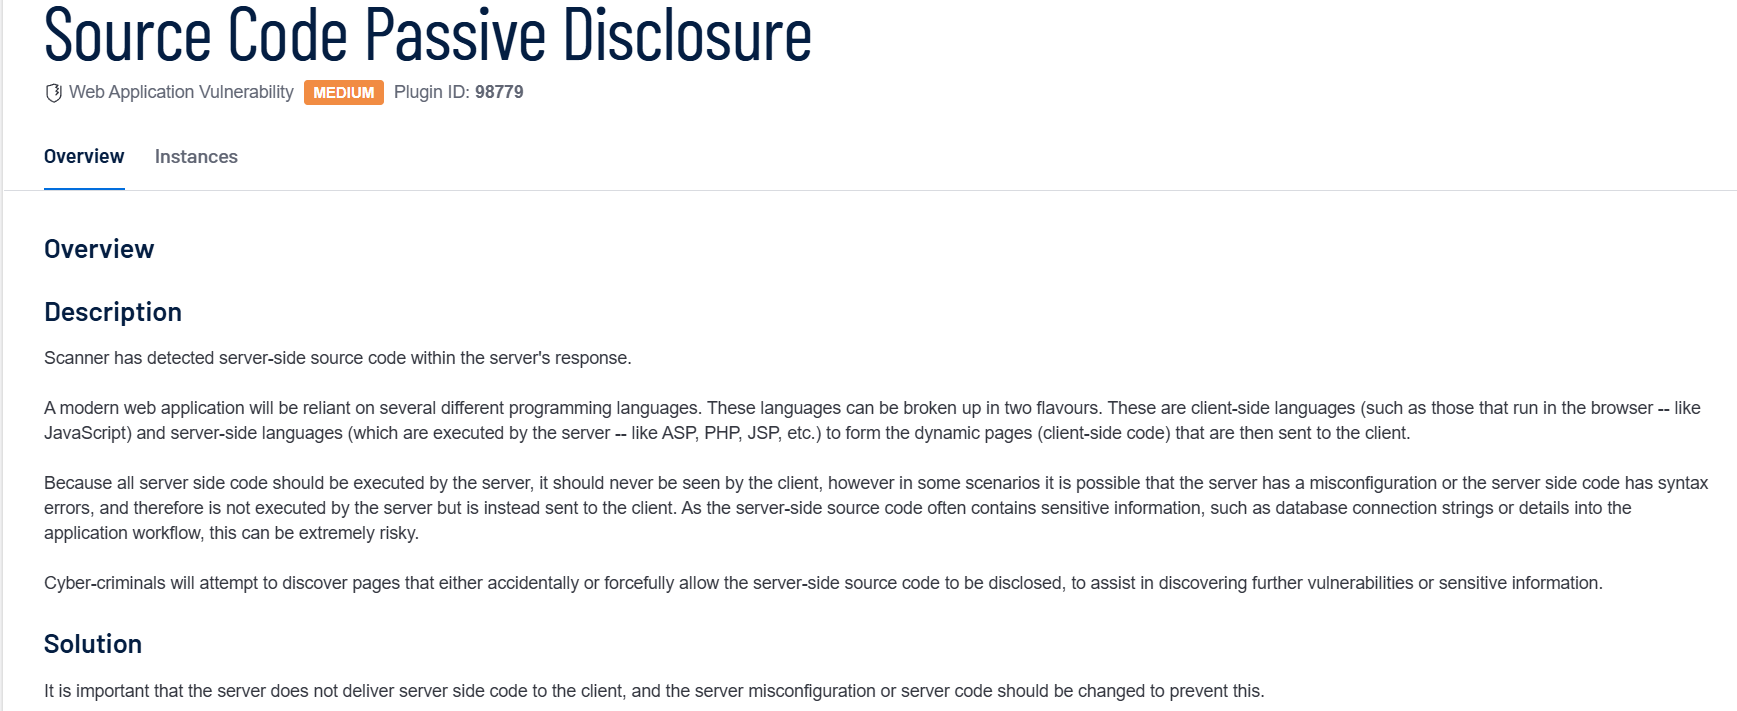
\includegraphics[width=0.8\textwidth]{assets/images-was/Vulnerabilidades Relacionadas a Configurações e Exposição de Informações/Exposição de Código e Recursos/Source Code Passive Disclosure.png}
                        \end{figure}
                        \FloatBarrier
                        \textbf{Descrição:} Foi detectada a divulgação passiva de código-fonte do lado do servidor na resposta do servidor. Aplicações web modernas utilizam diversas linguagens de programação que podem ser classificadas em duas categorias: linguagens do lado do cliente (executadas no navegador, como JavaScript) e linguagens do lado do servidor (executadas no servidor, como ASP, PHP, JSP, etc.), que formam as páginas dinâmicas enviadas ao cliente.

    Todo código do lado do servidor deve ser executado pelo servidor e nunca exposto ao cliente. No entanto, devido a configurações incorretas do servidor ou erros de sintaxe, pode ocorrer que o código do lado do servidor não seja executado e, em vez disso, seja enviado ao cliente. Como o código-fonte do lado do servidor frequentemente contém informações sensíveis, como strings de conexão de banco de dados ou detalhes sobre o fluxo de trabalho da aplicação, essa exposição representa um risco significativo.

    Criminosos cibernéticos podem tentar descobrir páginas que, acidentalmente ou propositalmente, permitem a divulgação do código-fonte do lado do servidor, a fim de identificar vulnerabilidades ou informações sensíveis.

\textbf{Solução:} É fundamental garantir que o servidor não entregue código do lado do servidor ao cliente. Para isso, deve-se corrigir a configuração incorreta do servidor ou ajustar o código do servidor para evitar essa exposição.

%---------------------------------------------------------------------------------
    \item

\textbf{Total de URIs Afetadas:} 1

\textbf{Instâncias Afetadas:}
\begin{itemize}
    \item \url{https://comunicacao.salvador.ba.gov.br}
\end{itemize}

%-------------- FIM DA VULNERABILIDADE Source Code Passive Disclosure --------------
\end{enumerate}
%-------------- FIM DA SUBCATEGORIA Exposição de Código e Recursos --------------
%-------------- FIM DA CATEGORIA Vulnerabilidades Relacionadas a Configurações e Exposição de Informações --------------
%-------------- INÍCIO DA CATEGORIA Vulnerabilidades Relacionadas a Injeção de Código --------------
\subsection{Vulnerabilidades Relacionadas a Injeção de Código}
Descrição não disponível.

%-------------- INÍCIO DA SUBCATEGORIA Cross-Site Scripting (XSS) --------------
\subsubsection{Cross-Site Scripting (XSS)}
Aqui são abordadas as vulnerabilidades XSS, onde atacantes conseguem injetar scripts maliciosos nas páginas da aplicação, podendo roubar dados de usuários ou realizar ações indesejadas em nome do usuário.

\begin{enumerate}
%-------------- INÍCIO DA VULNERABILIDADE jQuery 1.2.0 < 3.5.0 Cross-Site Scripting --------------
\item \textbf{jQuery 1.2.0 < 3.5.0 Cross-Site Scripting}

                        \begin{figure}[h!]
                        \centering
                        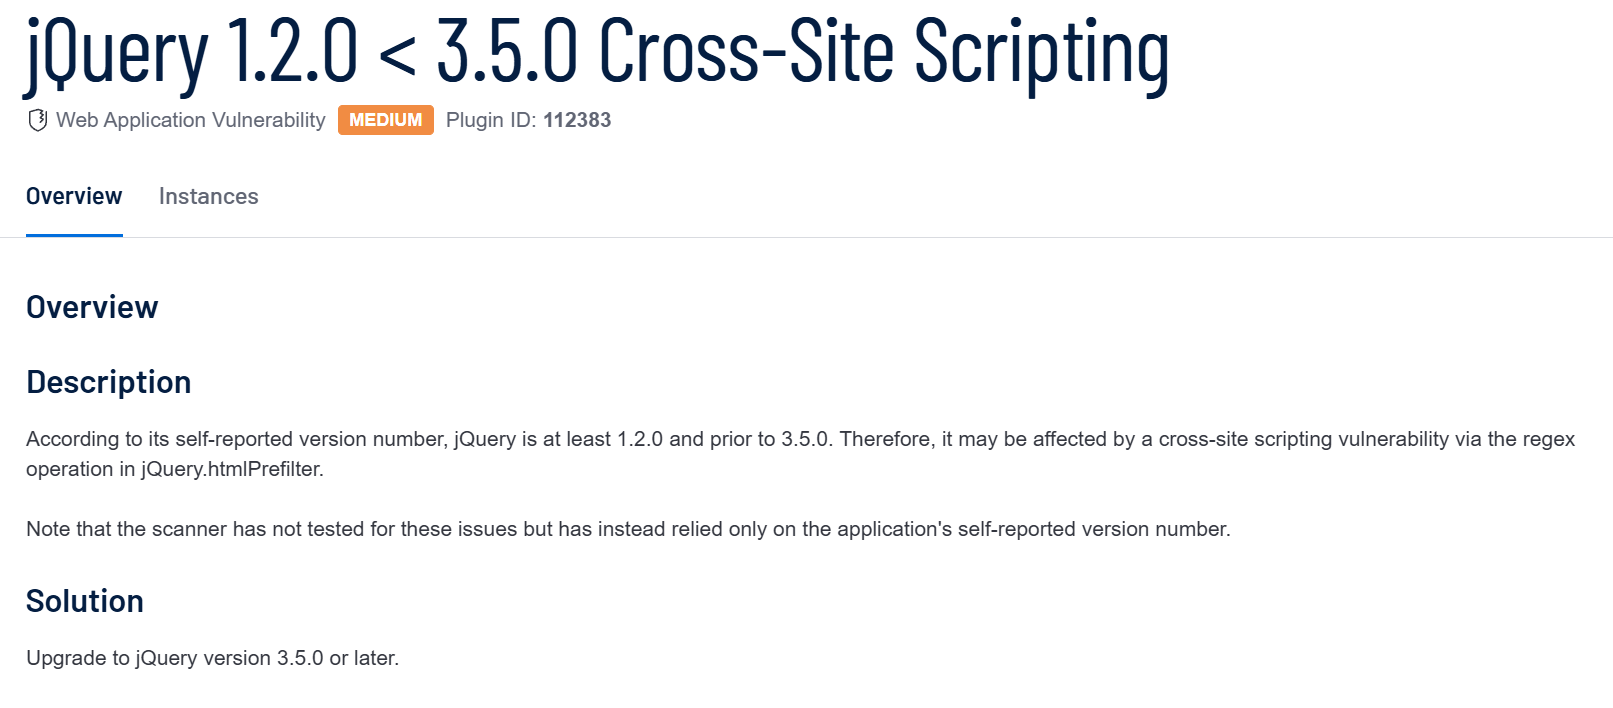
\includegraphics[width=0.8\textwidth]{assets/images-was/Vulnerabilidades Relacionadas a Injeção de Código/Cross-Site Scripting(XSS)/jQuery 1.2.0 inferior a 3.5.0 Cross-Site Scripting.png }
                        \end{figure}
                        \FloatBarrier
                        \textbf{Descrição:} De acordo com o número de versão autodeclarado, a versão do jQuery da aplicação é pelo menos 1.2.0 e anterior à 3.5.0. Nesse intervalo de versões, o jQuery pode ser vulnerável a um ataque de Cross-Site Scripting (XSS) devido a uma falha na operação de regex na função \texttt{jQuery.htmlPrefilter}. Essa falha pode ser explorada por um atacante para injetar e executar código JavaScript malicioso no contexto do navegador de um usuário, comprometendo a segurança da aplicação e dos dados do usuário.

    Vale ressaltar que o scanner não realizou um teste direto para identificar essa vulnerabilidade, mas confiou exclusivamente na versão informada pela aplicação.

\textbf{Solução:} A solução para essa vulnerabilidade é atualizar o jQuery para a versão 3.5.0 ou posterior, que resolve a falha de segurança relacionada ao \texttt{htmlPrefilter}. Essa atualização garantirá que a aplicação esteja protegida contra essa vulnerabilidade de XSS.

\textbf{Total de URIs Afetadas:} 3

\textbf{Instâncias Afetadas:}
\begin{itemize}
    \item \url{http://agenciadenoticias.salvador.ba.gov.br}
    \item \url{http://dom.salvador.ba.gov.br}
    \item \url{https://www.credenciamento.salvador.ba.gov.br}
\end{itemize}

%-------------- FIM DA VULNERABILIDADE jQuery 1.2.0 < 3.5.0 Cross-Site Scripting --------------
\end{enumerate}
%-------------- FIM DA SUBCATEGORIA Cross-Site Scripting (XSS) --------------
%-------------- INÍCIO DA SUBCATEGORIA Outras Injeções --------------
\subsubsection{Outras Injeções}
Descrição não disponível.

\begin{enumerate}
%-------------- INÍCIO DA VULNERABILIDADE HTML/CSS Injection --------------
\item \textbf{HTML/CSS Injection}

                        \begin{figure}[h!]
                        \centering
                        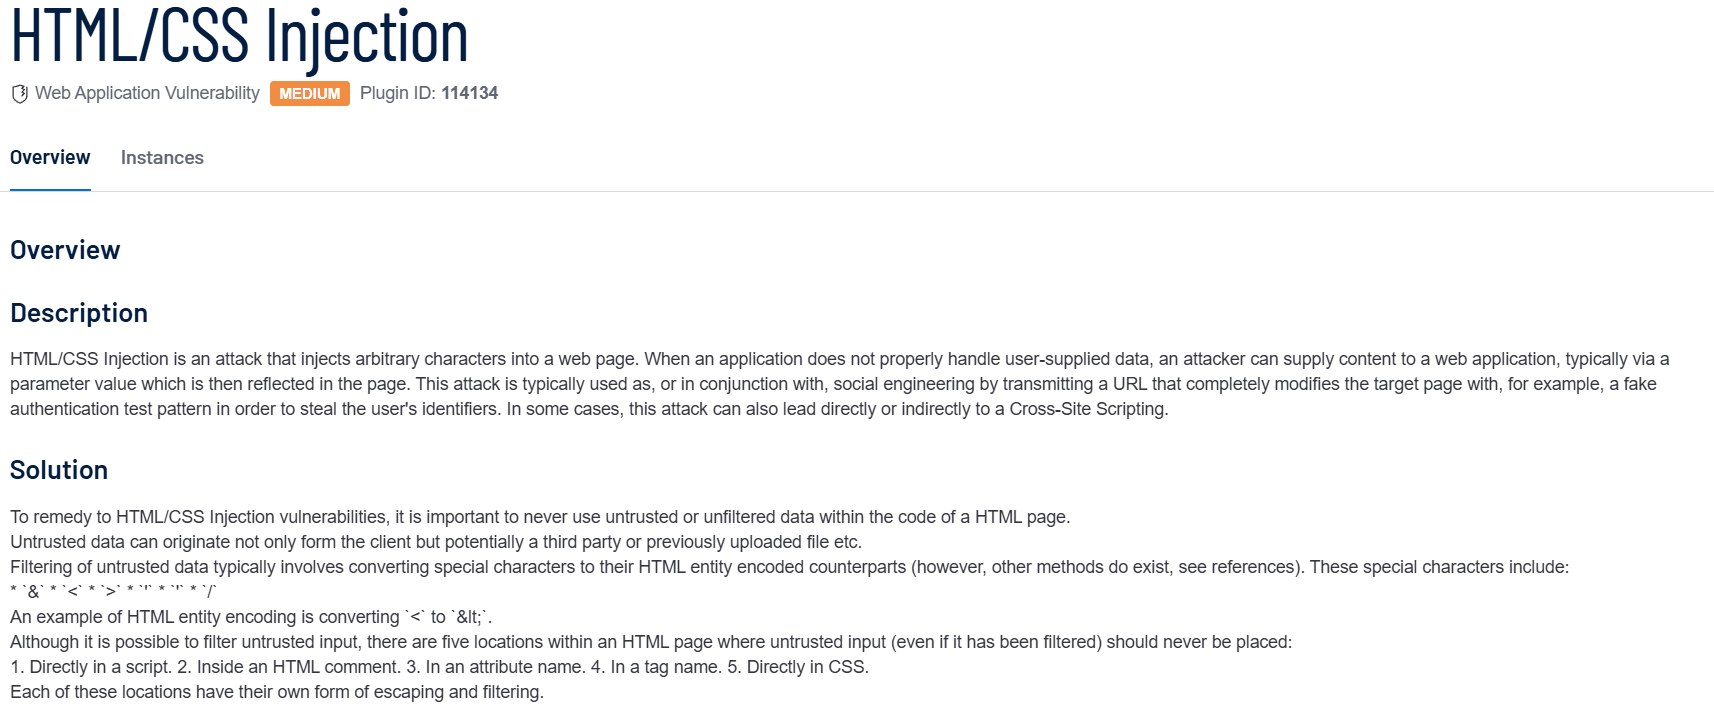
\includegraphics[width=0.8\textwidth]{assets/images-was/Vulnerabilidades Relacionadas a Injeção de Código/Outras Injeções/HTML-CSS Injection.png}
                        \end{figure}
                        \FloatBarrier
                        \textbf{Descrição:}  A injeção HTML/CSS é um ataque que injeta caracteres arbitrários em uma página web. Quando uma aplicação não lida corretamente com dados fornecidos pelo usuário, um atacante pode fornecer conteúdo a uma aplicação web, normalmente através de um valor de parâmetro que é refletido na página. Esse ataque é frequentemente usado como parte de engenharia social, transmitindo uma URL que modifica completamente a página alvo com, por exemplo, um padrão de teste de autenticação falso, para roubar os identificadores do usuário. Em alguns casos, esse ataque também pode levar, direta ou indiretamente, a um Cross-Site Scripting (XSS).


\textbf{Solução:} Para remediar as vulnerabilidades de injeção HTML/CSS, é importante nunca usar dados não confiáveis ou não filtrados dentro do código de uma página HTML.
Dados não confiáveis podem originar-se não apenas do cliente, mas também de terceiros ou de arquivos previamente carregados, entre outros.
A filtragem de dados não confiáveis normalmente envolve a conversão de caracteres especiais para suas versões codificadas em entidades HTML (no entanto, existem outros métodos, consulte as referências). Esses caracteres especiais incluem:
\begin{itemize}
    \item \texttt{\&}
    \item \texttt{<}
    \item \texttt{>}
    \item \texttt{\'}
    \item \texttt{\"}
    \item \texttt{/}
\end{itemize}
Um exemplo de codificação de entidades HTML é converter \texttt{<} para \texttt{\&lt;}.

Embora seja possível filtrar entradas não confiáveis, existem cinco locais dentro de uma página HTML onde a entrada não confiável (mesmo que filtrada) nunca deve ser colocada:
\begin{enumerate}
    \item Diretamente em um script.
    \item Dentro de um comentário HTML.
    \item Em um nome de atributo.
    \item Em um nome de tag.
    \item Diretamente em CSS.
\end{enumerate}
Cada um desses locais possui sua própria forma de escape e filtragem.

\textbf{Total de URIs Afetadas:} 2

\textbf{Instâncias Afetadas:}
\begin{itemize}
    \item \url{https://comunicacao.salvador.ba.gov.br}
    \item \url{https://www.credenciamento.salvador.ba.gov.br}
\end{itemize}

%-------------- FIM DA VULNERABILIDADE HTML/CSS Injection --------------
\end{enumerate}
%-------------- FIM DA SUBCATEGORIA Outras Injeções --------------
%-------------- FIM DA CATEGORIA Vulnerabilidades Relacionadas a Injeção de Código --------------
%-------------- INÍCIO DA CATEGORIA Vulnerabilidades em Cookies e Segurança de Sessão --------------
\subsection{Vulnerabilidades em Cookies e Segurança de Sessão}
Descrição não disponível.

%-------------- INÍCIO DA SUBCATEGORIA Vulnerabilidades em Cookies e Segurança de Sessão --------------
\subsubsection{Vulnerabilidades em Cookies e Segurança de Sessão}
Descrição não disponível.

\begin{enumerate}
%-------------- INÍCIO DA VULNERABILIDADE Cookie Without SameSite Flag Detected --------------
\item \textbf{Cookie Without SameSite Flag Detected}

                        \begin{figure}[h!]
                        \centering
                        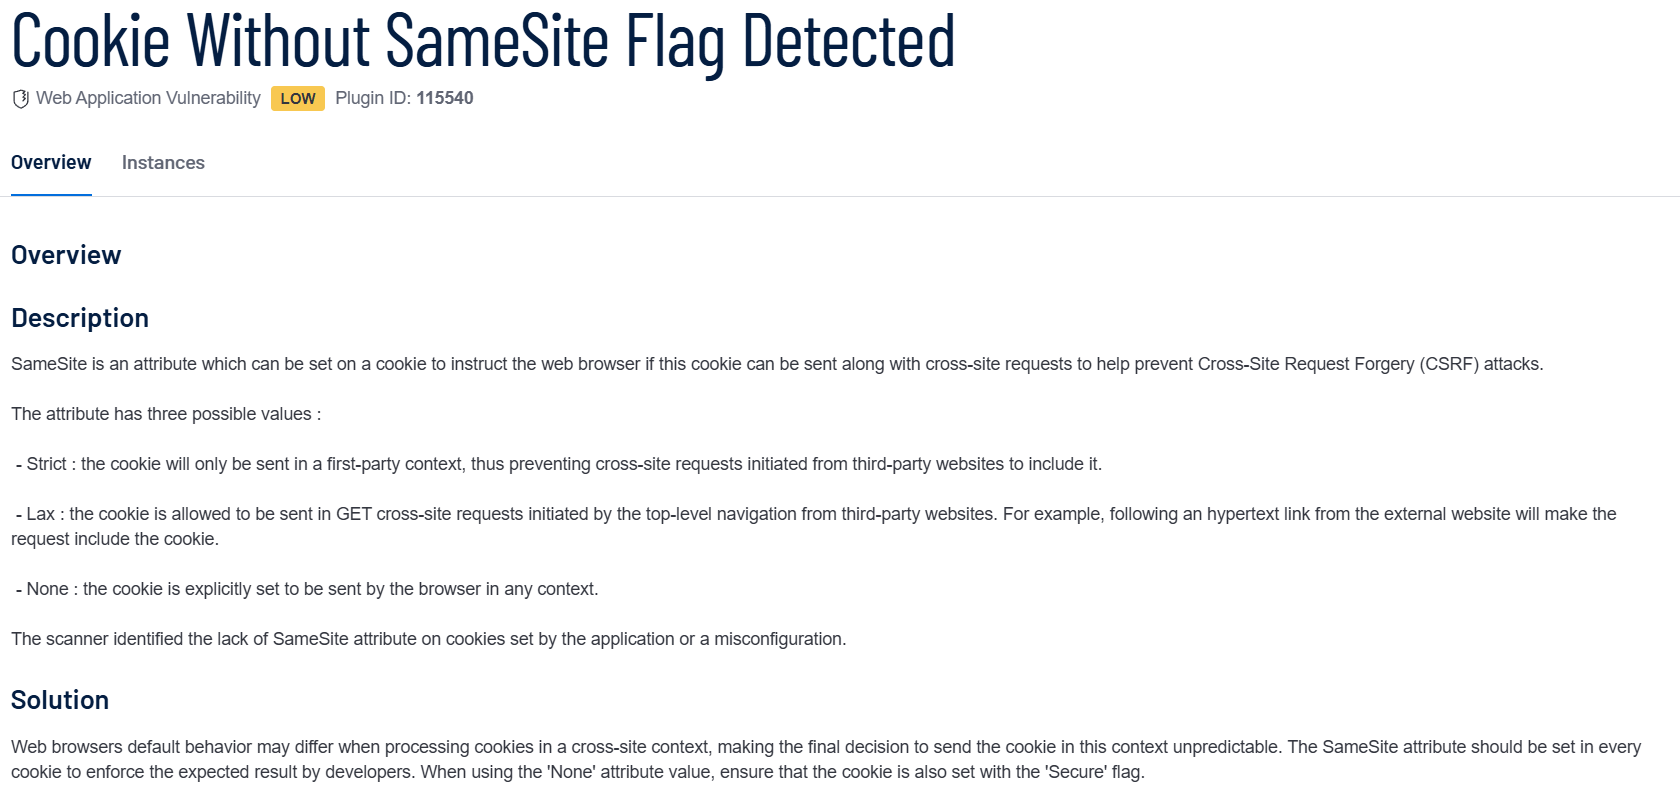
\includegraphics[width=0.8\textwidth]{assets/images-was/Vulnerabilidades em Cookies e Segurança de Sessão/Cookie Without SameSite Flag Detected.png}
                        \end{figure}
                        \FloatBarrier
                        \textbf{Descrição:} O atributo SameSite pode ser configurado em cookies para informar ao navegador se o cookie pode ser enviado junto com solicitações de sites diferentes (cross-site), ajudando a prevenir ataques de Cross-Site Request Forgery (CSRF). Esse atributo pode ter três valores possíveis:

    \begin{itemize}
    \item \textbf{Strict}: o cookie será enviado apenas em contextos de primeira parte, ou seja, apenas para o próprio site, impedindo que sites de terceiros o incluam em requisições.
    \item \textbf{Lax}: o cookie pode ser enviado em requisições GET de sites de terceiros, quando a navegação é iniciada pelo usuário em um link externo. Por exemplo, ao clicar em um link de um site externo, o cookie será incluído na solicitação.
    \item \textbf{None}: o cookie será explicitamente enviado pelo navegador em qualquer contexto, independentemente de ser uma requisição de primeira parte ou de terceiros.
    \end{itemize}

O scanner identificou que o aplicativo não configura ou configura incorretamente o atributo SameSite nos cookies. Isso pode resultar em um comportamento inesperado, já que o navegador pode, por padrão, enviar cookies em contextos cruzados, aumentando o risco de ataques CSRF.

\textbf{Solução:} Para mitigar essa vulnerabilidade, é essencial configurar o atributo SameSite em todos os cookies. O valor do atributo deve ser ajustado conforme o comportamento desejado. Ao usar o valor "None", é crucial também configurar o cookie com a flag \textit{Secure}, garantindo que ele seja enviado apenas por conexões HTTPS seguras.

\textbf{Total de URIs Afetadas:} 4

\textbf{Instâncias Afetadas:}
\begin{itemize}
    \item \url{http://agenciadenoticias.salvador.ba.gov.br}
    \item \url{https://comunicacao.salvador.ba.gov.br}
    \item \url{http://dom.salvador.ba.gov.br}
    \item \url{https://www.credenciamento.salvador.ba.gov.br}
\end{itemize}

%-------------- FIM DA VULNERABILIDADE Cookie Without SameSite Flag Detected --------------
%-------------- INÍCIO DA VULNERABILIDADE Cookie Without Secure Flag Detected --------------
\item \textbf{Cookie Without Secure Flag Detected}

                        \begin{figure}[h!]
                        \centering
                        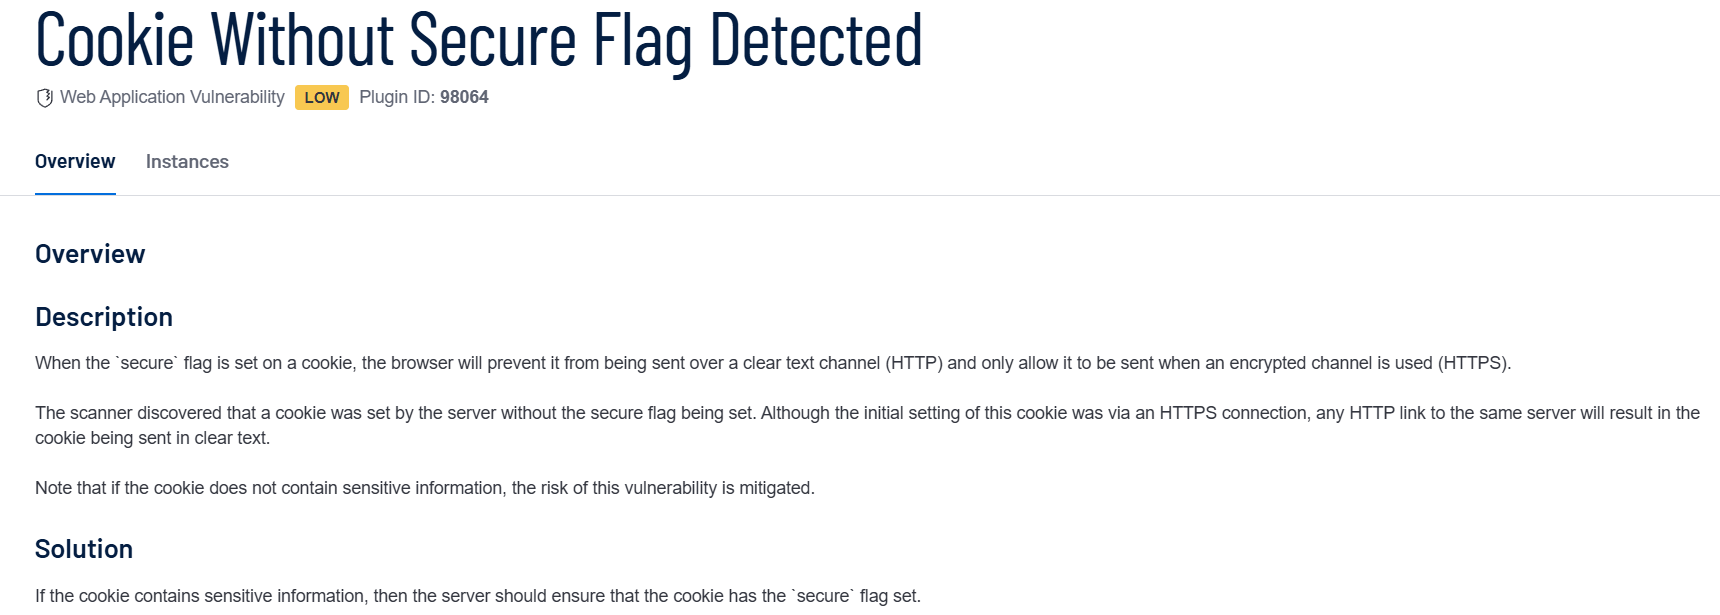
\includegraphics[width=0.8\textwidth]{assets/images-was/Vulnerabilidades em Cookies e Segurança de Sessão/Cookie Without Secure Flag Detected.png}
                        \end{figure}
                        \FloatBarrier
                        \textbf{Descrição:} Quando a flag secure é configurada em um cookie, o navegador impede que ele seja enviado através de um canal de texto claro (HTTP), permitindo que o cookie seja enviado apenas quando uma conexão segura (HTTPS) for utilizada. Isso ajuda a garantir que os cookies contendo informações sensíveis não sejam expostos em conexões não seguras.

O scanner detectou que o servidor configurou um cookie sem a flag secure. Embora o cookie tenha sido inicialmente configurado em uma conexão HTTPS, qualquer link HTTP para o mesmo servidor resultará no envio do cookie em texto claro, o que pode comprometer a segurança dos dados transmitidos, caso o cookie contenha informações sensíveis.

Vale ressaltar que, se o cookie não contiver informações sensíveis, o risco dessa vulnerabilidade é reduzido.

\textbf{Solução:} Se o cookie contiver informações sensíveis, como credenciais de usuário, dados financeiros ou informações pessoais, é essencial que o servidor configure o cookie com a flag secure. Isso garantirá que o cookie seja transmitido apenas em conexões HTTPS, protegendo assim a integridade e confidencialidade dos dados.

\textbf{Total de URIs Afetadas:} 3

\textbf{Instâncias Afetadas:}
\begin{itemize}
    \item \url{https://comunicacao.salvador.ba.gov.br}
    \item \url{http://dom.salvador.ba.gov.br}
    \item \url{https://www.credenciamento.salvador.ba.gov.br}
\end{itemize}

%-------------- FIM DA VULNERABILIDADE Cookie Without Secure Flag Detected --------------
%-------------- INÍCIO DA VULNERABILIDADE Cookie Without HttpOnly Flag Detected --------------
\item \textbf{Cookie Without HttpOnly Flag Detected}

                        \begin{figure}[h!]
                        \centering
                        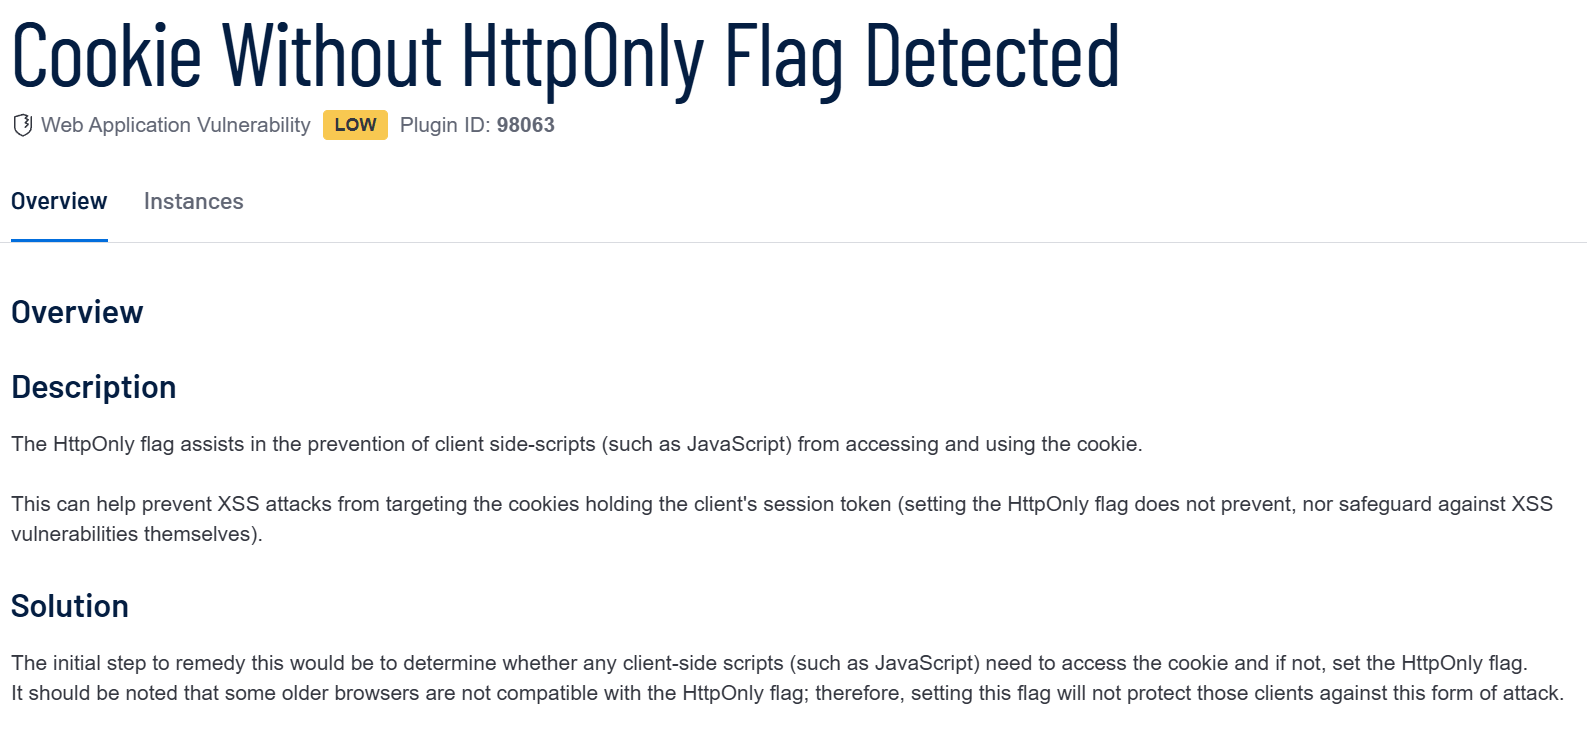
\includegraphics[width=0.8\textwidth]{assets/images-was/Vulnerabilidades em Cookies e Segurança de Sessão/Cookie Without HttpOnly Flag Detected.png}
                        \end{figure}
                        \FloatBarrier
                        \textbf{Descrição:} A flag \texttt{HttpOnly} ajuda a prevenir que scripts do lado do cliente (como o JavaScript) acessem e usem o cookie. Isso é particularmente importante para proteger os cookies que contêm tokens de sessão do cliente, já que impede que um script malicioso, como um que explora uma vulnerabilidade de Cross-Site Scripting (XSS), possa roubar esses dados sensíveis.

Vale destacar que configurar a flag \texttt{HttpOnly} não previne ou resolve vulnerabilidades XSS diretamente, mas limita o escopo de exploração ao impedir que os cookies sejam acessados por scripts do lado do cliente.

\textbf{Solução:} O primeiro passo para corrigir essa vulnerabilidade é determinar se algum script do lado do cliente (como o JavaScript) precisa acessar o cookie. Se o cookie não precisar ser acessado por scripts, a flag \texttt{HttpOnly} deve ser configurada. Essa configuração ajuda a proteger os dados do cookie contra tentativas de roubo por meio de ataques XSS.

É importante observar que navegadores mais antigos podem não ser compatíveis com a flag \texttt{HttpOnly}, o que significa que esses clientes ainda estarão suscetíveis a esse tipo de ataque, mesmo com a configuração da flag.

\textbf{Total de URIs Afetadas:} 3

\textbf{Instâncias Afetadas:}
\begin{itemize}
    \item \url{https://comunicacao.salvador.ba.gov.br}
    \item \url{http://dom.salvador.ba.gov.br}
    \item \url{https://www.credenciamento.salvador.ba.gov.br}
\end{itemize}

%-------------- FIM DA VULNERABILIDADE Cookie Without HttpOnly Flag Detected --------------
\end{enumerate}
%-------------- FIM DA SUBCATEGORIA Vulnerabilidades em Cookies e Segurança de Sessão --------------
%-------------- FIM DA CATEGORIA Vulnerabilidades em Cookies e Segurança de Sessão --------------
%-------------- INÍCIO DA CATEGORIA Outras Vulnerabilidades Críticas e Explorações --------------
\subsection{Outras Vulnerabilidades Críticas e Explorações}
Descrição não disponível.

%-------------- INÍCIO DA SUBCATEGORIA Desafios de Configuração de Segurança --------------
\subsubsection{Desafios de Configuração de Segurança}
Descrição não disponível.

\begin{enumerate}
%-------------- INÍCIO DA VULNERABILIDADE HTTP to HTTPS Redirect Not Enabled --------------
\item \textbf{HTTP to HTTPS Redirect Not Enabled}

                        \begin{figure}[h!]
                        \centering
                        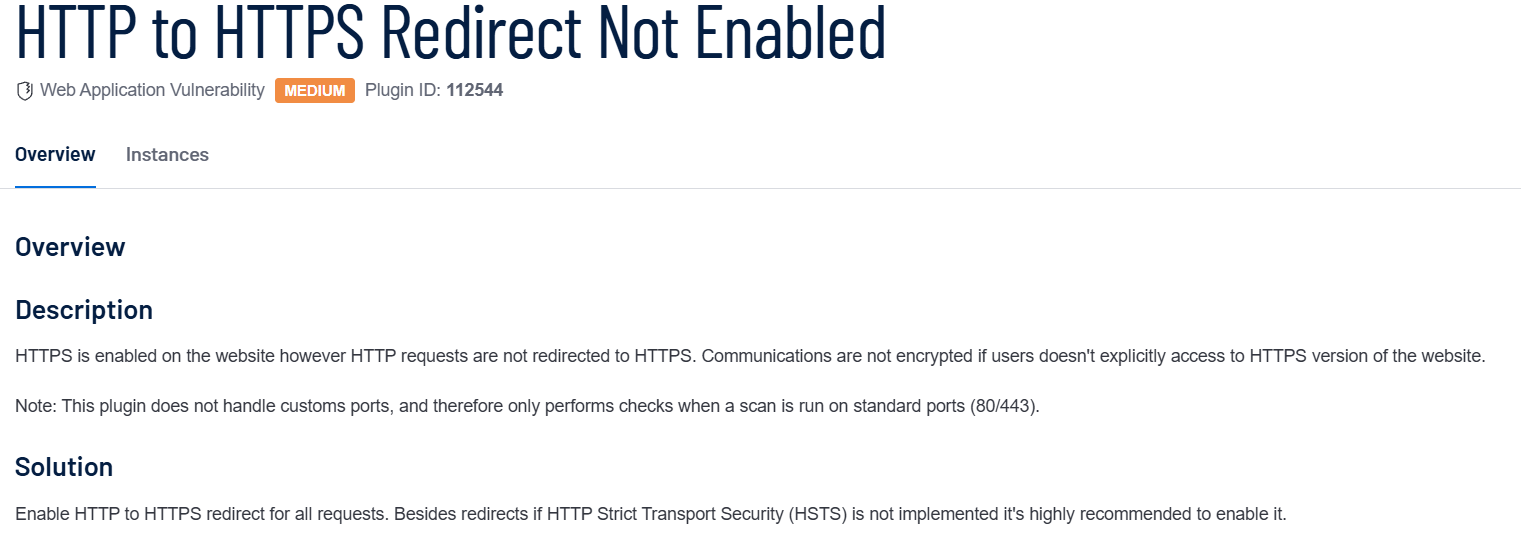
\includegraphics[width=0.8\textwidth]{assets/images-was/Outras Vulnerabilidades Críticas e Explorações/Desafios de Configuração de Segurança/HTTP to HTTPS Redirect Not Enabled.png}
                        \end{figure}
                        \FloatBarrier
                        \textbf{Descrição:} O HTTPS está habilitado no site, no entanto, as requisições HTTP não são redirecionadas para HTTPS. Isso significa que a comunicação não será criptografada se os usuários não acessarem explicitamente a versão HTTPS do site.

\textbf{Solução:} Habilite o redirecionamento de HTTP para HTTPS para todas as requisições. Além dos redirecionamentos, se o HTTP Strict Transport Security (HSTS) não estiver implementado, é altamente recomendado ativá-lo.

\textbf{Total de URIs Afetadas:} 4

\textbf{Instâncias Afetadas:}
\begin{itemize}
    \item \url{http://agenciadenoticias.salvador.ba.gov.br}
    \item \url{http://gct.salvador.ba.gov.br}
    \item \url{http://dom.salvador.ba.gov.br}
    \item \url{https://www.credenciamento.salvador.ba.gov.br}
\end{itemize}

%-------------- FIM DA VULNERABILIDADE HTTP to HTTPS Redirect Not Enabled --------------
%-------------- INÍCIO DA VULNERABILIDADE Permissive Content Security Policy Detected --------------
\item \textbf{Permissive Content Security Policy Detected}

                        \begin{figure}[h!]
                        \centering
                        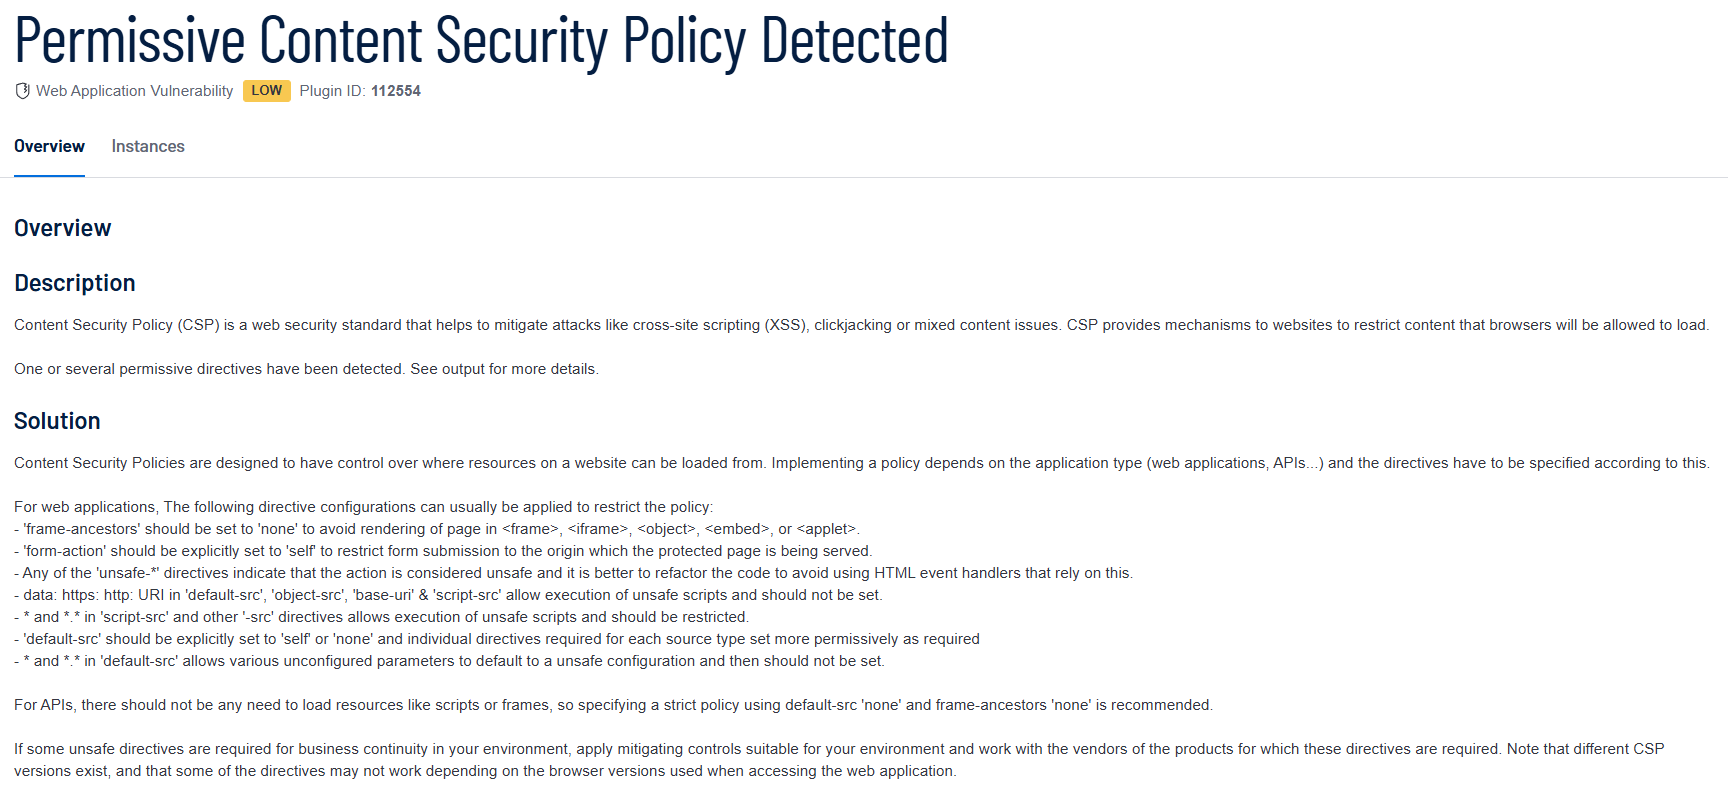
\includegraphics[width=0.8\textwidth]{assets/images-was/Outras Vulnerabilidades Críticas e Explorações/Desafios de Configuração de Segurança/Permissive Content Security Policy Detected.png}
                        \end{figure}
                        \FloatBarrier
                        \textbf{Descrição:} A Política de Segurança de Conteúdo (CSP) é um padrão de segurança da web que ajuda a mitigar ataques como Cross-Site Scripting (XSS), clickjacking ou problemas de conteúdo misto. O CSP permite que os sites controlem quais recursos os navegadores podem carregar, restringindo o conteúdo carregado e aumentando a proteção contra ataques.

No entanto, uma política de CSP excessivamente permissiva pode permitir que conteúdos não seguros sejam carregados, o que enfraquece a eficácia da política. O scanner identificou uma ou mais diretivas permissivas na política de CSP do site, o que pode expor o site a ataques como injeção de scripts maliciosos (XSS), carregamento de conteúdo inseguro ou execução de código não autorizado.

As diretivas permissivas podem incluir, por exemplo, o uso de * ou *.* nas diretrizes de fontes (como script-src ou default-src), o que permite a execução de scripts ou o carregamento de recursos de origens não confiáveis. Isso pode comprometer a segurança da aplicação ao permitir a execução de código arbitrário proveniente de fontes não autorizadas.

\textbf{Solução:} Para corrigir essa vulnerabilidade, recomenda-se restringir a política de CSP e aplicar as diretivas de forma mais rígida. A seguir, estão algumas diretrizes gerais que podem ser implementadas:

- Defina frame-ancestors como none para evitar que a página seja renderizada dentro de <frame>, <iframe>, <object>, <embed> ou <applet>.
- Configure form-action explicitamente como self para restringir o envio de formulários apenas à origem do site.
- Evite o uso das diretivas unsafe-*, pois indicam ações inseguras. Refatore o código para não depender de manipuladores de eventos HTML que utilizem essas diretivas.
- Evite o uso de data:, https: ou http: nas diretivas default-src, object-src, base-uri e script-src, pois essas configurações permitem a execução de scripts não seguros.
- Não utilize * ou *.* em diretivas como script-src e outras diretrizes -src, pois isso permite a execução de scripts não seguros de origens não especificadas.
- Defina default-src explicitamente como self ou none, e defina as diretivas individuais de forma mais permissiva apenas quando necessário.
- Para APIs, deve-se evitar carregar recursos como scripts ou frames. Use uma política rígida com default-src 'none' e frame-ancestors 'none'.

Se for necessário usar algumas diretivas inseguras para a continuidade dos negócios, aplique controles mitigadores adequados ao seu ambiente e consulte os fornecedores dos produtos que exigem essas diretivas. Lembre-se de que existem versões diferentes do CSP e que algumas diretivas podem não ser suportadas em versões de navegador mais antigas.

\textbf{Total de URIs Afetadas:} 1

\textbf{Instâncias Afetadas:}
\begin{itemize}
    \item \url{https://comunicacao.salvador.ba.gov.br}
\end{itemize}

%-------------- FIM DA VULNERABILIDADE Permissive Content Security Policy Detected --------------
\end{enumerate}
%-------------- FIM DA SUBCATEGORIA Desafios de Configuração de Segurança --------------
%-------------- INÍCIO DA SUBCATEGORIA Redirecionamentos e Autenticação --------------
\subsubsection{Redirecionamentos e Autenticação}
Descrição não disponível.

\begin{enumerate}
%-------------- INÍCIO DA VULNERABILIDADE Password Field With Auto-Complete --------------
\item \textbf{Password Field With Auto-Complete}

                        \begin{figure}[h!]
                        \centering
                        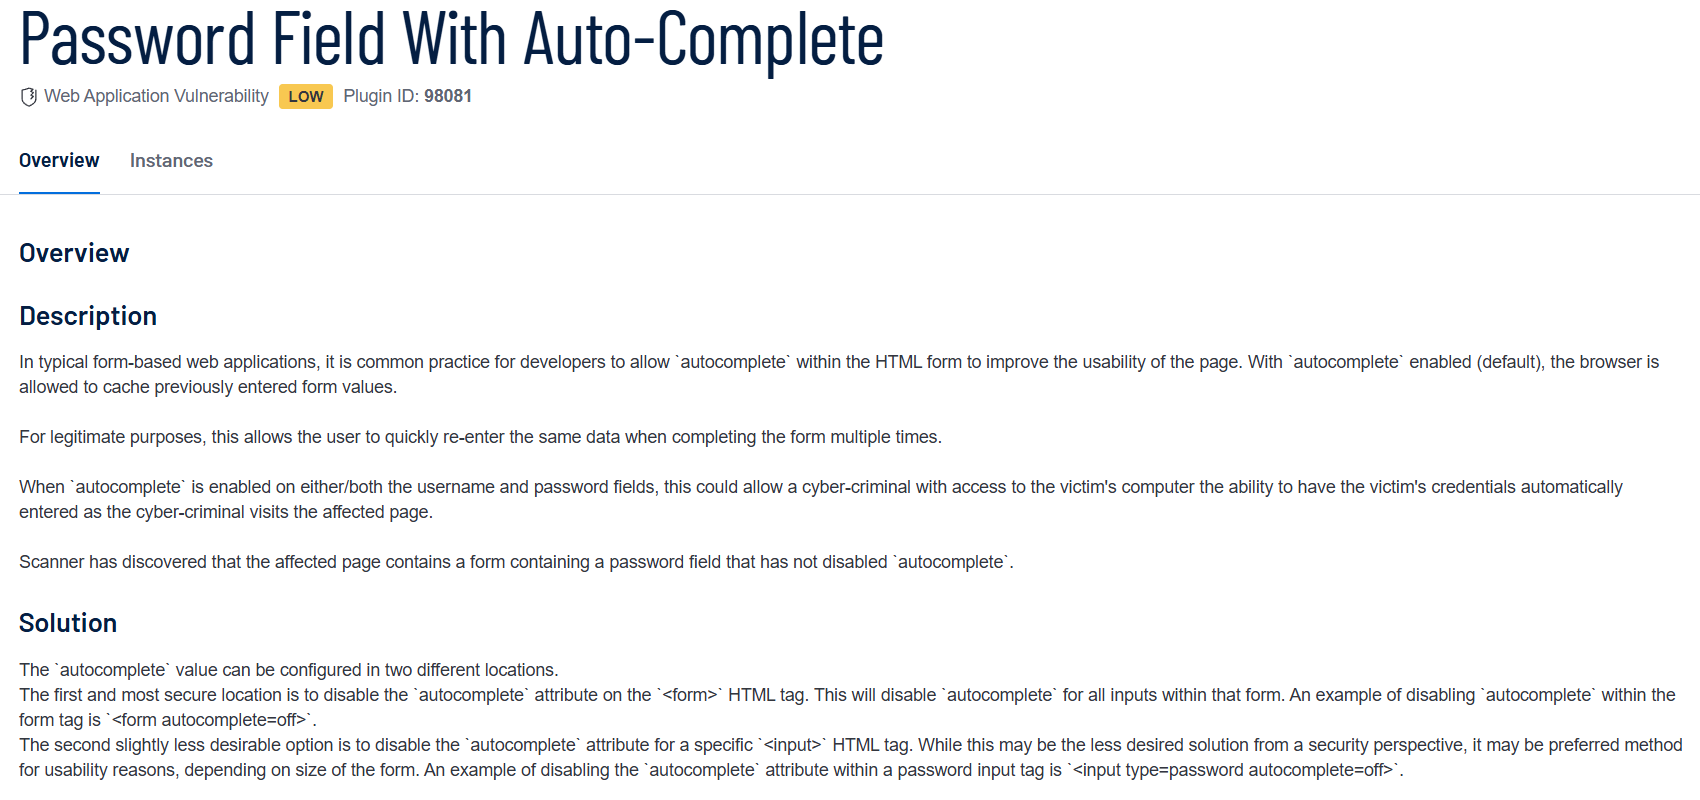
\includegraphics[width=0.8\textwidth]{assets/images-was/Outras Vulnerabilidades Críticas e Explorações/Redirecionamentos e Autenticação/Password Field With Auto-Complete.png}
                        \end{figure}
                        \FloatBarrier
                        \textbf{Descrição:} A vulnerabilidade Password Field With Auto-Complete ocorre quando um formulário de login permite que os navegadores completem automaticamente os campos de nome de usuário e senha, armazenando as credenciais do usuário localmente para reutilização. Isso pode ocorrer quando o atributo autocomplete não está desativado no campo de senha ou no formulário em si.
Em um cenário normal, o recurso de preenchimento automático é útil para facilitar o preenchimento de formulários. No entanto, se o preenchimento automático estiver habilitado em um campo de senha, um atacante que tenha acesso físico ao computador da vítima poderá visualizar e capturar as credenciais armazenadas, simplesmente acessando a página de login. Além disso, se o computador estiver comprometido por malware, esse recurso pode ser explorado para roubo de senhas.

O impacto dessa vulnerabilidade é elevado, pois pode expor as credenciais dos usuários a ataques locais. Esse risco é agravado se o dispositivo da vítima não estiver adequadamente protegido por medidas de segurança, como criptografia de dados e autenticação de múltiplos fatores.

\textbf{Solução:} Para mitigar essa vulnerabilidade, é recomendado desabilitar o preenchimento automático (autocomplete) nos campos de senha e em todo o formulário de login. Isso pode ser feito da seguinte maneira:

- Desabilitar o atributo autocomplete no elemento <form>, o que desativará o preenchimento automático para todos os campos do formulário: <form autocomplete="off">
- Desabilitar o atributo autocomplete no campo de senha especificamente, caso o preenchimento automático precise ser habilitado para outros campos do formulário: <input type="password" autocomplete="off">

Adotar essas práticas ajudará a reduzir o risco de exposição das credenciais armazenadas localmente em dispositivos comprometidos ou acessados indevidamente.

\textbf{Total de URIs Afetadas:} 3

\textbf{Instâncias Afetadas:}
\begin{itemize}
    \item \url{http://agenciadenoticias.salvador.ba.gov.br}
    \item \url{http://dom.salvador.ba.gov.br}
    \item \url{https://www.credenciamento.salvador.ba.gov.br}
\end{itemize}

%-------------- FIM DA VULNERABILIDADE Password Field With Auto-Complete --------------
\end{enumerate}
%-------------- FIM DA SUBCATEGORIA Redirecionamentos e Autenticação --------------
%-------------- INÍCIO DA SUBCATEGORIA Redirecionamentos e Autênticação --------------
\subsubsection{Redirecionamentos e Autênticação}
Descrição não disponível.

\begin{enumerate}
%-------------- INÍCIO DA VULNERABILIDADE Login Form Cross-Site Request Forgery --------------
\item \textbf{Login Form Cross-Site Request Forgery}

                        \begin{figure}[h!]
                        \centering
                        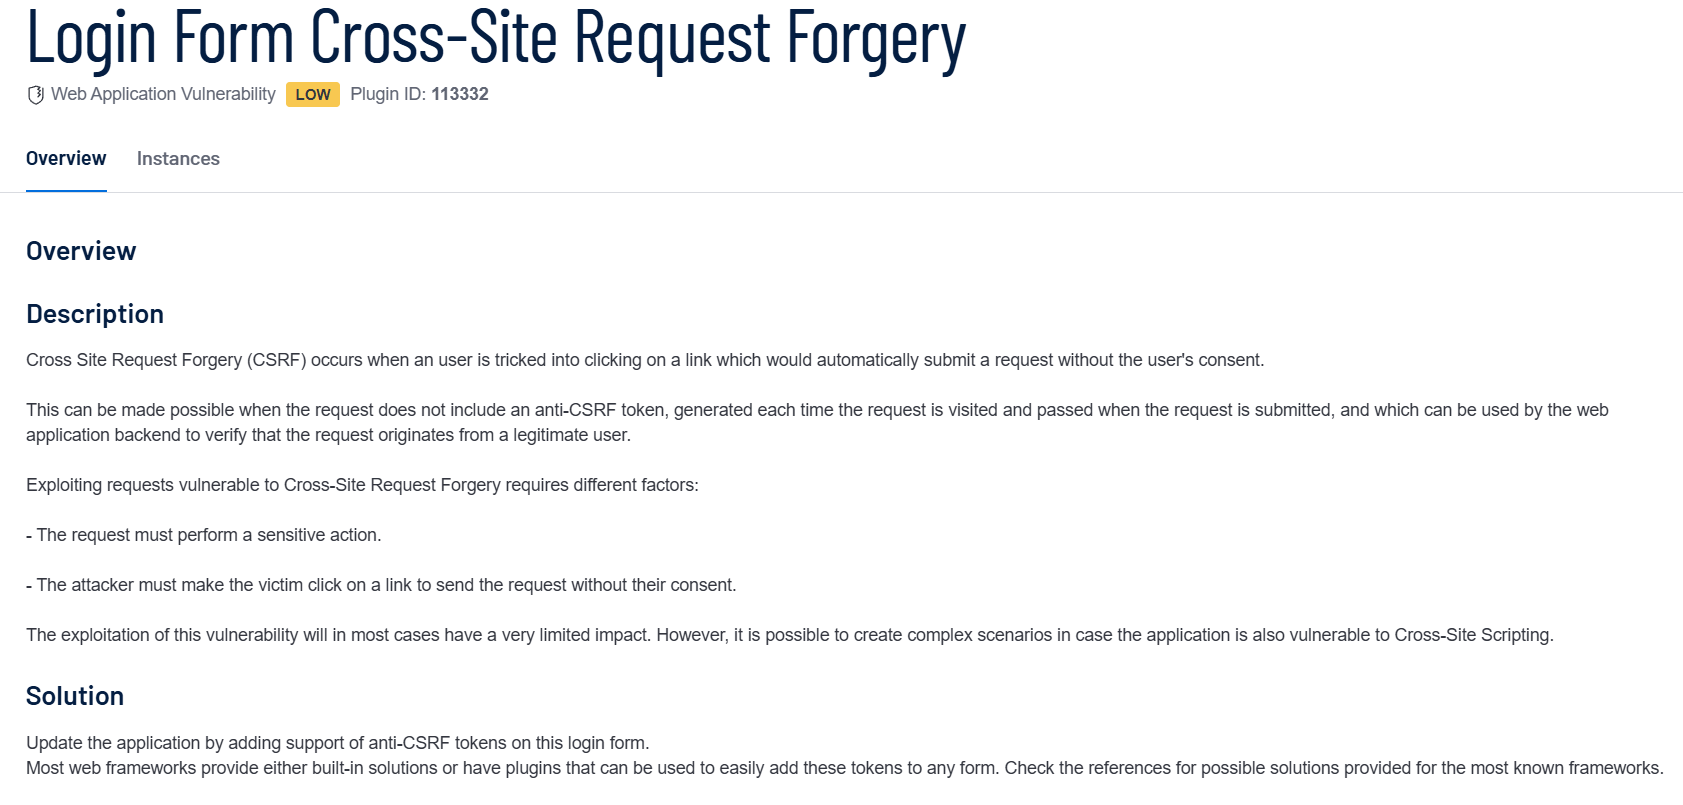
\includegraphics[width=0.8\textwidth]{assets/images-was/Outras Vulnerabilidades Críticas e Explorações/Redirecionamentos e Autenticação/Login Form Cross-Site Request Forgery.png}
                        \end{figure}
                        \FloatBarrier
                        \textbf{Descrição:} A vulnerabilidade de Cross-Site Request Forgery (CSRF) ocorre quando um usuário é induzido a clicar em um link que automaticamente submete uma solicitação sem o seu consentimento. Isso pode acontecer quando a solicitação não inclui um token anti-CSRF, gerado a cada visita e passado na submissão da solicitação. O backend da aplicação utiliza esse token para verificar se a requisição é originada de um usuário legítimo.

    Para que uma requisição vulnerável ao CSRF seja explorada, alguns fatores devem estar presentes:
    \begin{itemize}
        \item A requisição deve realizar uma ação sensível.
        \item O atacante deve induzir a vítima a clicar em um link que envie a requisição sem consentimento.
    \end{itemize}
    
    O impacto da exploração dessa vulnerabilidade costuma ser limitado, mas cenários complexos podem ser criados caso a aplicação também esteja vulnerável a Cross-Site Scripting (XSS).

\textbf{Solução:} Atualize a aplicação para incluir tokens anti-CSRF nesse formulário de login. A maioria dos frameworks web oferece soluções embutidas ou plugins que facilitam a adição desses tokens a qualquer formulário. Consulte as referências para possíveis soluções nos frameworks mais conhecidos.

\textbf{Total de URIs Afetadas:} 2

\textbf{Instâncias Afetadas:}
\begin{itemize}
    \item \url{http://dom.salvador.ba.gov.br}
    \item \url{https://www.credenciamento.salvador.ba.gov.br}
\end{itemize}

%-------------- FIM DA VULNERABILIDADE Login Form Cross-Site Request Forgery --------------
%-------------- INÍCIO DA VULNERABILIDADE Unencrypted Password Form --------------
\item \textbf{Unencrypted Password Form}

                        \begin{figure}[h!]
                        \centering
                        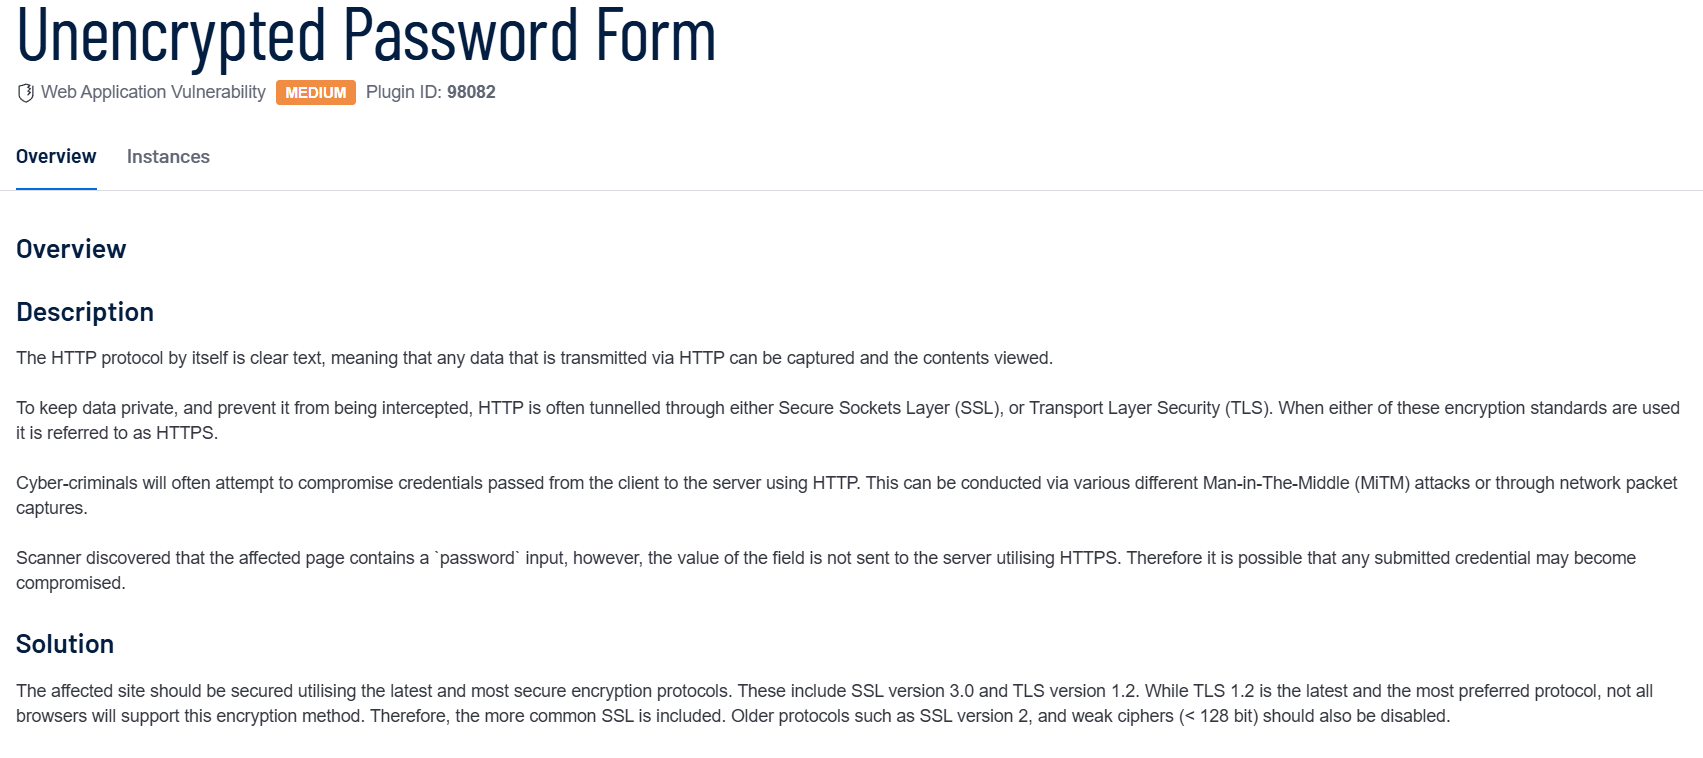
\includegraphics[width=0.8\textwidth]{assets/images-was/Outras Vulnerabilidades Críticas e Explorações/Redirecionamentos e Autenticação/Unencrypted Password Form.png}
                        \end{figure}
                        \FloatBarrier
                        \textbf{Descrição:} O protocolo HTTP é transmitido em texto claro, o que significa que qualquer dado enviado por meio de HTTP pode ser capturado e visualizado. Para proteger dados e evitar que sejam interceptados, o HTTP pode ser encapsulado em Secure Sockets Layer (SSL) ou Transport Layer Security (TLS), passando a ser conhecido como HTTPS.

    Criminosos cibernéticos frequentemente tentam comprometer credenciais transmitidas entre o cliente e o servidor usando HTTP, através de ataques de Man-in-the-Middle (MiTM) ou captura de pacotes de rede. O scanner detectou que a página afetada contém um campo de entrada de senha (`password`), mas o valor desse campo não é transmitido ao servidor com o uso de HTTPS. Dessa forma, existe a possibilidade de que as credenciais enviadas sejam comprometidas.

\textbf{Solução:} O site afetado deve ser protegido utilizando os protocolos de criptografia mais recentes e seguros, como SSL versão 3.0 e TLS versão 1.2. Embora o TLS 1.2 seja o mais atual e preferido, nem todos os navegadores oferecem suporte a esse método de criptografia, portanto, o uso de SSL também é recomendado. Protocolos antigos, como SSL versão 2, e cifras fracas (inferiores a 128 bits) devem ser desativados.

\textbf{Total de URIs Afetadas:} 2

\textbf{Instâncias Afetadas:}
\begin{itemize}
    \item \url{http://agenciadenoticias.salvador.ba.gov.br}
    \item \url{http://dom.salvador.ba.gov.br}
\end{itemize}

%-------------- FIM DA VULNERABILIDADE Unencrypted Password Form --------------
\end{enumerate}
%-------------- FIM DA SUBCATEGORIA Redirecionamentos e Autênticação --------------
%-------------- INÍCIO DA SUBCATEGORIA Versões Antigas e Falhas de Plugins --------------
\subsubsection{Versões Antigas e Falhas de Plugins}
Descrição não disponível.

\begin{enumerate}
%-------------- INÍCIO DA VULNERABILIDADE jQuery < 3.4.0 Prototype Pollution --------------
\item \textbf{jQuery < 3.4.0 Prototype Pollution}

                        \begin{figure}[h!]
                        \centering
                        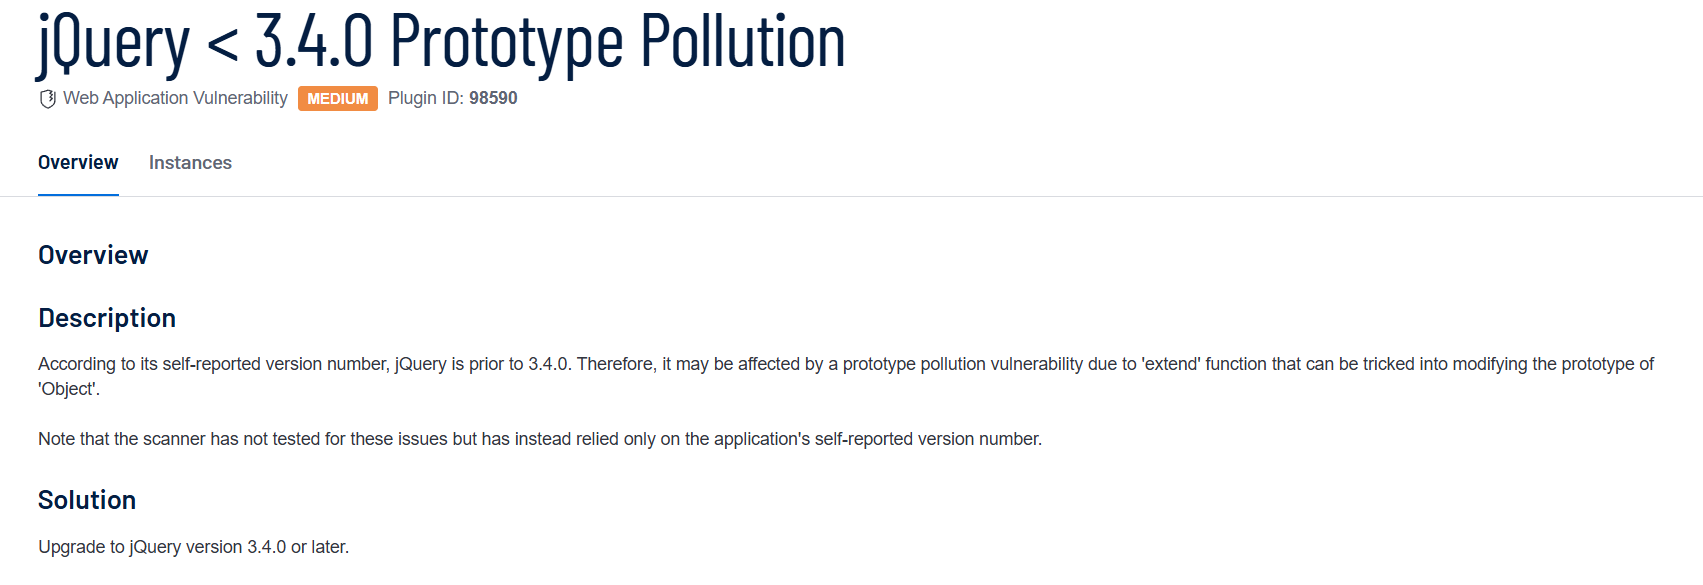
\includegraphics[width=0.8\textwidth]{assets/images-was/Outras Vulnerabilidades Críticas e Explorações/Versões Antigas e Falhas de Plugins/jQuery inferior 3.4.0 Prototype Pollution}
                        \end{figure}
                        \FloatBarrier
                        \textbf{Descrição:} De acordo com o número de versão informado, o jQuery está em uma versão anterior à 3.4.0. Portanto, ele pode ser afetado por uma vulnerabilidade de poluição de protótipo devido à função 'extend', que pode ser enganada para modificar o protótipo de 'Object'.

Observe que o scanner não testou diretamente essas questões, confiando apenas no número da versão informado pela aplicação.

\textbf{Solução:} Atualize para a versão 3.4.0 ou posterior do jQuery.

\textbf{Total de URIs Afetadas:} 3

\textbf{Instâncias Afetadas:}
\begin{itemize}
    \item \url{http://agenciadenoticias.salvador.ba.gov.br}
    \item \url{http://dom.salvador.ba.gov.br}
    \item \url{https://www.credenciamento.salvador.ba.gov.br}
\end{itemize}

%-------------- FIM DA VULNERABILIDADE jQuery < 3.4.0 Prototype Pollution --------------
%-------------- INÍCIO DA VULNERABILIDADE jQuery 1.4.0 < 1.12.0 Cross-Site Scripting --------------
\item \textbf{jQuery 1.4.0 < 1.12.0 Cross-Site Scripting}

                        \begin{figure}[h!]
                        \centering
                        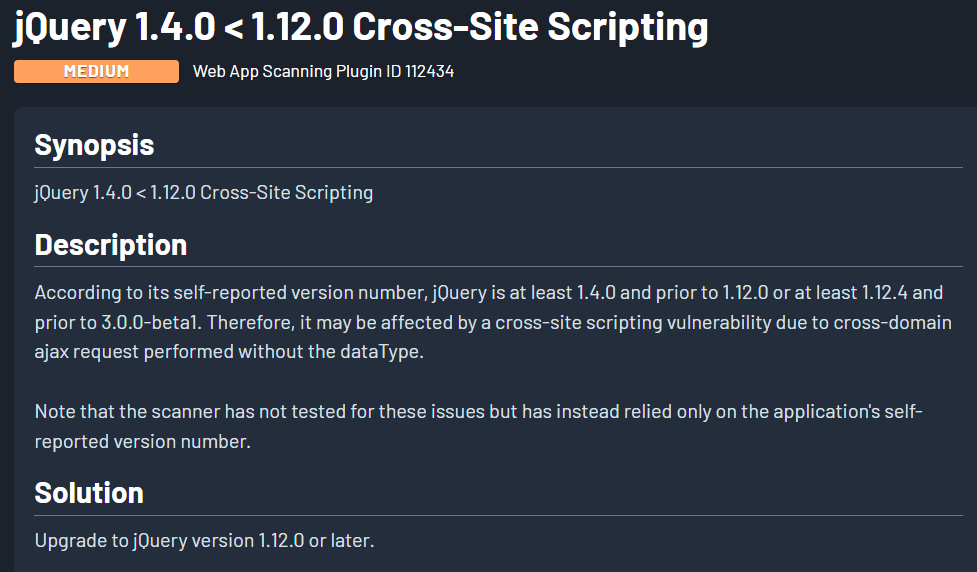
\includegraphics[width=0.8\textwidth]{assets/images-was/Outras Vulnerabilidades Críticas e Explorações/Versões Antigas e Falhas de Plugins/jQuery 1.4.0-1.12.0 Cross-Site Scripting.png}
                        \end{figure}
                        \FloatBarrier
                        \textbf{Descrição:} De acordo com o número da versão auto-relatado, o jQuery está na versão pelo menos 1.4.0 e anterior à 1.12.0 ou pelo menos 1.12.4 e anterior à 3.0.0-beta1. Portanto, ele pode ser afetado por uma vulnerabilidade de Cross-Site Scripting (XSS) devido a requisições ajax entre domínios realizadas sem o parâmetro dataType. Observa-se que o scanner não testou diretamente essas questões, mas baseou-se apenas na versão auto-relatada pela aplicação.

\textbf{Solução:} Atualize para a versão 1.12.0 ou posterior do jQuery.

\textbf{Total de URIs Afetadas:} 3

\textbf{Instâncias Afetadas:}
\begin{itemize}
    \item \url{http://agenciadenoticias.salvador.ba.gov.br}
    \item \url{http://dom.salvador.ba.gov.br}
    \item \url{https://www.credenciamento.salvador.ba.gov.br}
\end{itemize}

%-------------- FIM DA VULNERABILIDADE jQuery 1.4.0 < 1.12.0 Cross-Site Scripting --------------
%-------------- INÍCIO DA VULNERABILIDADE jQuery < 1.9.0 Cross-Site Scripting --------------
\item \textbf{jQuery < 1.9.0 Cross-Site Scripting}

                        \begin{figure}[h!]
                        \centering
                        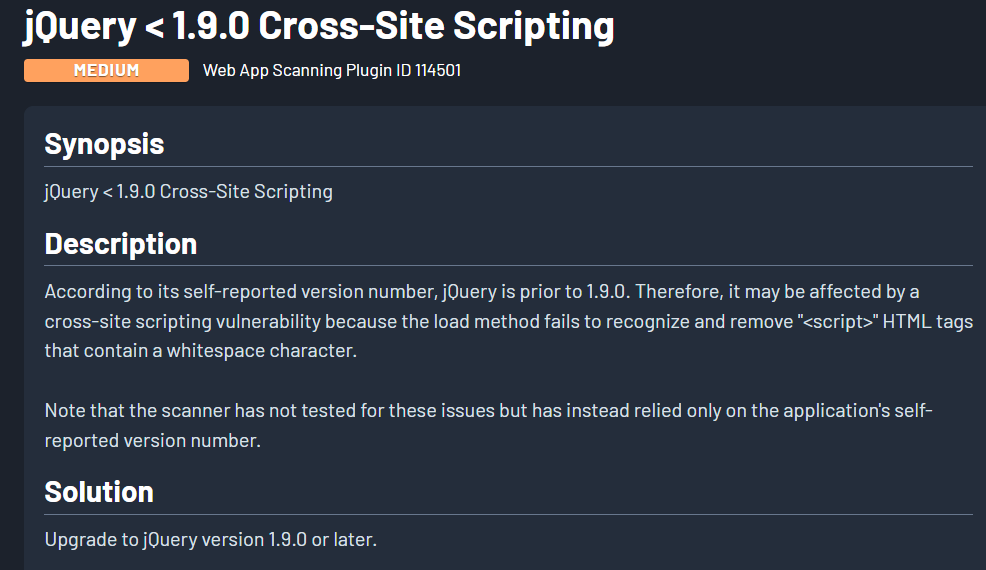
\includegraphics[width=0.8\textwidth]{assets/images-was/Outras Vulnerabilidades Críticas e Explorações/Versões Antigas e Falhas de Plugins/jQuery-1.9.0.png}
                        \end{figure}
                        \FloatBarrier
                        \textbf{Descrição:} De acordo com o número de versão auto-relatado, o jQuery está em uma versão anterior à 1.9.0. Portanto, ele pode ser afetado por uma vulnerabilidade de Cross-Site Scripting (XSS), pois o método 'load' falha ao reconhecer e remover corretamente as tags '<script>' que contêm um caractere de espaço.

    Note que o scanner não testou essas questões, mas confiou apenas no número da versão auto-relatado pela aplicação.

\textbf{Solução:} Atualize para a versão 1.9.0 ou posterior do jQuery.

\textbf{Total de URIs Afetadas:} 2

\textbf{Instâncias Afetadas:}
\begin{itemize}
    \item \url{http://agenciadenoticias.salvador.ba.gov.br}
    \item \url{https://www.credenciamento.salvador.ba.gov.br}
\end{itemize}

%-------------- FIM DA VULNERABILIDADE jQuery < 1.9.0 Cross-Site Scripting --------------
%-------------- INÍCIO DA VULNERABILIDADE PHP Unsupported Version --------------
\item \textbf{PHP Unsupported Version}

                        \begin{figure}[h!]
                        \centering
                        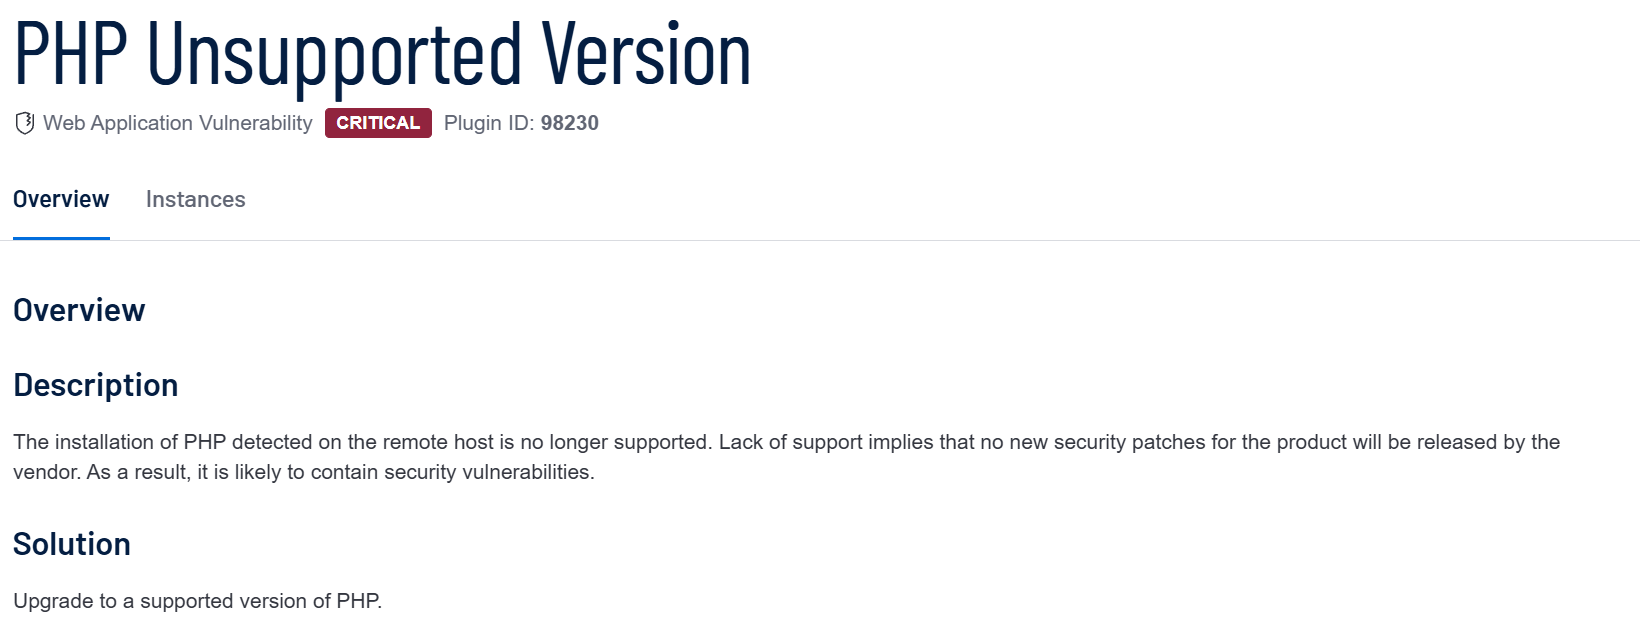
\includegraphics[width=0.8\textwidth]{assets/images-was/Outras Vulnerabilidades Críticas e Explorações/Versões Antigas e Falhas de Plugins/PHP Unsupported Version.png}
                        \end{figure}
                        \FloatBarrier
                        \textbf{Descrição:} A instalação do PHP detectada no host remoto não é mais suportada. A falta de suporte implica que nenhuma nova correção de segurança será liberada pelo fornecedor, o que aumenta a probabilidade de a versão instalada conter vulnerabilidades de segurança.

\textbf{Solução:} Atualize para uma versão suportada do PHP.

\textbf{Total de URIs Afetadas:} 1

\textbf{Instâncias Afetadas:}
\begin{itemize}
    \item \url{http://dom.salvador.ba.gov.br}
\end{itemize}

%-------------- FIM DA VULNERABILIDADE PHP Unsupported Version --------------
\end{enumerate}
%-------------- FIM DA SUBCATEGORIA Versões Antigas e Falhas de Plugins --------------
%-------------- FIM DA CATEGORIA Outras Vulnerabilidades Críticas e Explorações --------------
%-------------- INÍCIO DAS VULNERABILIDADES SEM CATEGORIA --------------
\section{Vulnerabilidades sem Categoria}
\begin{itemize}
    \item Apache 2.4.x < 2.4.58 Multiple Vulnerabilities
    \item Apache 2.4.x < 2.4.56 Multiple Vulnerabilities
    \item Apache 2.4.x < 2.4.49 Multiple Vulnerabilities
    \item Apache 2.4.x < 2.4.55 Multiple Vulnerabilities
    \item Apache 2.4.x < 2.4.52 Multiple Vulnerabilities
    \item Apache 2.4.x < 2.4.46 Multiple Vulnerabilities
    \item Apache 2.4.x < 2.4.43 Multiple Vulnerabilities
    \item Apache 2.4.x < 2.4.60 Multiple Vulnerabilities
    \item Apache 2.4.x < 2.4.62 Multiple Vulnerabilities
    \item Apache 2.4.x < 2.4.59 Multiple Vulnerabilities
    \item Apache 2.4.x < 2.4.39 Multiple Vulnerabilities
    \item Apache 2.4.x < 2.4.48 Multiple Vulnerabilities
    \item Apache 2.4.x < 2.4.54 Multiple Vulnerabilities
    \item Apache 2.4.x < 2.4.41 Multiple Vulnerabilities
    \item Apache 2.4.x < 2.4.53 Multiple Vulnerabilities
    \item Apache Tomcat 7.0.x < 7.0.99 Session Fixation
    \item Apache Tomcat 7.0.x < 7.0.107 Information Disclosure
    \item Apache Tomcat 7.0.x < 7.0.108 Multiple Vulnerabilities
    \item Apache Tomcat 7.0.0 < 7.0.85 Security Constraint Weakness
    \item Apache Tomcat 7.0.23 < 7.0.91 Open Redirect
    \item Apache Tomcat 7.0.x < 7.0.81 Multiple Vulnerabilities
    \item Apache Tomcat 7.0.x < 7.0.100 Multiple Vulnerabilities
    \item Apache Tomcat 7.0.x < 7.0.109 Authentication Weakness
    \item Apache Tomcat 7.0.x < 7.0.77 Information Disclosure
    \item Apache Tomcat 7.0.x < 7.0.104 Multiple Vulnerabilities
    \item Apache Tomcat 7.0.25 < 7.0.90 Multiple Vulnerabilities
    \item Apache Tomcat 7.0.0 < 7.0.94 Remote Code Execution on Windows
    \item Apache Tomcat 7.0.28 < 7.0.88 Denial of Service
    \item Apache Tomcat Unsupported Version
    \item Apache Tomcat 7.0.x < 7.0.78 Remote Error Page Manipulation
    \item CVS/SVN User Disclosure
    \item Apache Tomcat 7.0.x < 7.0.82 Remote Code Execution via JSP Upload
    \item Apache Tomcat 7.0.x < 7.0.99 Local Privilege Escalation
    \item Apache Tomcat 7.0.x < 7.0.105 Denial of Service
    \item Disclosed Hong Kong Identity Number
    \item DOM-based Cross-Site Scripting (XSS)
    \item Apache Tomcat Default Files
    \item Apache Tomcat Manager Detected
    \item Cross-Site Scripting (XSS) in HTML tag
\end{itemize}
%-------------- FIM DAS VULNERABILIDADES SEM CATEGORIA --------------

%-------------- FIM DA CATEGORIA Outras Vulnerabilidades Críticas e Explorações --------------
\section{Conclusão}

A auditoria de segurança cibernética realizada pela Gerência Especial de Segurança da Informação da COGEL revelou um cenário alarmante de vulnerabilidades e riscos no ambiente de aplicações e servidores da Prefeitura de Salvador, administrado pela  Secretaria de Saúde - SMS. Foram identificadas diversas vulnerabilidades ativas, incluindo falhas críticas, altas, médias e baixas, que expõem o ambiente a possíveis ataques cibernéticos. Problemas graves, permissões incorretas de aplicações, suporte a protocolos e cifras criptográficas inseguras, e configurações inseguras em Sistemas Operacionais para aplicações críticas e a utilização de sistemas não suportados foram destacados.\\

A presença dessas vulnerabilidades representa uma ameaça significativa à segurança da informação e à continuidade dos serviços da Prefeitura de Salvador. A adoção de políticas de segurança mais rigorosas e a conformidade com normas como ISO/IEC 27001, NIST SP 800-53 e PCI DSS são essenciais para fortalecer a postura de segurança cibernética da instituição. A urgência na aplicação de patches e na implementação de medidas corretivas é imperativa para mitigar esses riscos e proteger a integridade, confidencialidade e disponibilidade dos serviços e dados da prefeitura e de seus cidadãos.\\

Por atingir seu objetivo, esta comissão encerra o presente instrumento ao tempo que declara o fim da Auditoria de Segurança Cibernética — Ambiente da Secretaria de Saúde - SMS.

\vfill % Isso preenche o espaço vazio antes da assinatura

\begin{flushright}
\textbf{Salvador, Dezembro de 2023 \\
Gerência Especial de Segurança da Informação \\
Diretoria Técnica e de Infraestrutura \\
Companhia de Governança Eletrônica do Salvador}
\end{flushright}


\end{document}
